\documentclass{article}

% AAAI-27 submission format. The submission option anonymizes the title block
% and suppresses author metadata for double-blind review.
\usepackage[submission]{aaai2027}

\usepackage{graphicx}
\usepackage{tabularx}
\usepackage{booktabs}
\usepackage{amsmath,amssymb}
\usepackage[table]{xcolor}
\usepackage{tcolorbox}
\tcbuselibrary{skins,breakable}
\usepackage{multirow}

\tcbset{
  taskprompt/.style={
    enhanced,
    colback=gray!4,
    colframe=gray!55,
    fonttitle=\bfseries\small,
    coltitle=black,
    boxrule=0.4pt,
    arc=2pt,
    left=4pt, right=4pt, top=3pt, bottom=3pt,
    before skip=0pt,
    after skip=0pt,
  },
  rubricbox/.style={
    enhanced,
    colback=blue!3,
    colframe=blue!40!black,
    fonttitle=\bfseries\small,
    coltitle=white,
    boxrule=0.4pt,
    arc=2pt,
    left=4pt, right=4pt, top=3pt, bottom=3pt,
    before skip=0pt,
    after skip=0pt,
  },
  outputbox gpt/.style={
    enhanced, breakable,
    colback=green!4,
    colframe=green!45!black,
    fonttitle=\bfseries\small,
    coltitle=white,
    boxrule=0.4pt,
    arc=2pt,
    left=4pt, right=4pt, top=3pt, bottom=3pt,
    before skip=0pt,
    after skip=0pt,
    title=#1,
  },
    outputbox ds/.style={
    enhanced, breakable,
    colback=cyan!6!white,
    colframe=cyan!60!blue,
    fonttitle=\bfseries\small,
    coltitle=white,
    boxrule=0.4pt,
    arc=2pt,
    left=4pt, right=4pt, top=3pt, bottom=3pt,
    before skip=0pt,
    after skip=0pt,
    title=#1,
  },
}

% -------------------------------------------------
% Citations
% -------------------------------------------------
\usepackage[round,authoryear]{natbib}

% Keep the submission source free of author, affiliation, contact, and date
% metadata. The AAAI submission style renders the title block anonymously.
\title{CentaurBench: Benchmarking LLM Assistance on Real-world Work}
\author{Anonymous submission}
\affiliations{}

\begin{document}

\maketitle

\begin{abstract}
Most LLM benchmarks rank models on their ability to automate work tasks. In practice, however, models are often used to assist other (human or LLM) agents. The question that drives model selection is therefore not only which model produces the best output, but which model most improves the work of another (weaker) agent. We introduce a unified framework that evaluates the capability of models to automate and augment another agent's performance. Across seven economically grounded real-world tasks, an assistant model writes assistance text for a standardized lower-capacity worker model, which produces the deliverable. In automation mode, the assistant produces the output directly. Outputs are scored through blind pairwise comparisons by an LLM judge panel with task-specific rubrics, replicated across ten runs. Rankings across the two regimes are only modestly correlated, and the automation winner loses augmentation on five of seven tasks. Assistance is not reliably positive. The unaided worker outranks every assisted condition on three tasks, and only one model's guidance beats no guidance on average.  These results suggest that automation ability is an incomplete proxy for assistance quality, motivating benchmarks that evaluate models according to the roles they play in human-AI and multi-agent systems. 



%Most LLM benchmarks rank models on their ability to automate work tasks. In practice, however, models are often used to assist other (human or LLM) agents. The question that drives model selection is therefore not only which model produces the best output, but which model most improves the work of another (weaker) agent. We introduce a unified framework that evaluates the capability of models to automate and augment another agent's performance. Across seven economically grounded real-world tasks, an assistant model writes assistance text for a standardized lower-capacity worker model, which produces the deliverable. In automation mode, the assistant produces the output directly. Outputs are scored through blind pairwise comparisons by an LLM judge panel with task-specific rubrics, replicated across ten runs. The two regimes produce vastly different rankings: model-level rank correlation is $\rho = 0.48$, and the automation winner loses augmentation on five of seven tasks. Assistance is not reliably positive. The unaided worker outranks every assisted condition on three tasks, and only one model's guidance beats no guidance on average.  These results suggest that automation ability is an incomplete proxy for assistance quality, motivating benchmarks that evaluate models according to the roles they play in human-AI and multi-agent systems.

% We consider seven economically grounded practical work tasks spanning structured planning, analytical work, and human-facing services. For each task, in augmentation mode, an assistant model produces assistance text that is passed to a standardized lower-capacity worker model that produces the output. In automation  mode, the assistant model also produces the output on the same task without coordinating with another agent. Every output is scored through blind pairwise comparisons by a panel of LLM judges on a customized rubric, with rankings replicated across ten independent runs.






%% OLD %%



%Most LLM benchmarks rank models on a single ability: how well a model completes a task on its own. But that is often not how AI is used in practice. Frequently, a stronger model assists another agent, either a human worker or a weaker assistant model by providing guidance on task planning and execution, while the other agent produces the final output. The question that drives model selection is therefore not only which model produces the best output, but which model most improves the work of another agent. These are distinct capabilities, and we understand little about how models compare on the capability to assist another agent. We introduce a unified framework that evaluates the capability of models for automation as well as augmentation for another agent's performance on real world tasks. 

%We consider seven economically grounded practical work tasks spanning structured planning, analytical work, and human-facing services. For each task, in augmentation mode, an assistant model produces assistance text (a plan, checklist, and self-review), that is passed to a standardized lower-capacity worker model that produces the output. In automation  mode, the same model also produces the output on the same task without coordinating with another agent. 

%Every output is scored through blind pairwise comparisons by a panel of LLM judges on a customized rubric, with rankings replicated across ten independent runs. 

%Automation and augmentation produce substantially different rankings: model-level rank correlation between regimes is ρ = 0.48, and the automation winner loses the augmentation regime on five of seven tasks. Assistance is not reliably positive — the unaided worker outranks every assisted condition on three of seven tasks, and only one model's guidance beats no guidance on average. Reversals can be extreme: the best automation model on one task is among the worst assistants on the same task. Direct task-solving ability is an incomplete proxy for assistance value; the relevant question for human-in-the-loop and multi-agent systems is not "which model is best?" but "which model, in which role, on which task?"


%Our main result suggests that automation and augmentation produce substantially different rankings. 
%On five of seven tasks, the model that is dominates in automation mode, does not win in augmentation mode. Further, on three of seven tasks, the worker models output worsens with assistance rather than improving. More generally, while automation rankings are concentrated and consistent with conventional capability orderings, augmentation rankings are more dispersed and task-dependent. No assistant dominates across tasks, and several strong direct solvers perform relatively poorly as assistants. These findings suggest that direct task-solving ability (automation) is an incomplete proxy for assistance quality (augmentation). For human-in-the-loop and multi-agent systems, our framework provides an alternate way to guage model capabilities that take into account the role and tasks at hand.
\end{abstract}



\section{Introduction}

    
Since the explosion in the adoption of large language models (LLMs), researchers have sought to measure the growth in capabilities across a wide variety of benchmarks. This work has moved from measuring capabilities on abstract knowledge or capabilities \citep{hendrycks2021, srivastava2023} to more real-world, economically valuable tasks \citep{gdpval2025, profbench2025, occubench2026}. These benchmarks provide an excellent indication of a model's capacity to automate work. However, in many real organizational and personal settings, models do not produce the output themselves. They are often assisting other agents, such as a human or another, perhaps weaker, LLM to complete the task. In such settings, models help workers plan an approach, decompose a task into steps, identify potential errors, and revise their work while leaving responsibility for the final deliverable with the worker. A model that excels at completing a task independently may not be the model that provides the most useful guidance to someone else. Put differently, as research with humans shows, the best (AI) player may not be the best coach \citep{hinds1999, camerer1989}. 


% Yet, almost without exception, most benchmarks measure only a single dimension of the model as an autonomous task solver or how well a model completes a task on its own. In organizational settings, however, models are also used as assistants. They help workers plan an approach, decompose a task into steps, identify potential errors, and revise their work while leaving responsibility for the final deliverable with the worker. A model that excels at completing a task independently may not be the model that provides the most useful guidance to someone else. Put differently, the best player may not be the best coach.

%% we should also cite andy and erik's centaur benchpaper upfront. 
Existing research does not provide a general way to compare these two capabilities. On the one hand, large-scale computer science benchmarks primarily rank models as autonomous task solvers, including increasingly realistic evaluations of professional and economically valuable work \citep{hendrycks2021, liang2023, gdpval2025, sopbench2025, occubench2026, profbench2025, jobbench2026}. On the other hand, field experiments by economists and management scholars examine whether AI augments human performance, but generally evaluate a single model in a particular domain and against a limited set of experimental conditions \citep{noy2023, peng2023, dellacqua2023, chen2024, doshi2024, brynjolfsson2025, ju2026}. 

There is a line of work on multi-agent systems. In one stream, past work finds that a model's performance in isolation does not reliably predict its performance in interactive settings \citep{collins2024, chang2025, vaccaro2024}. Research has also studied how stronger models can teach weaker agents \citep{saha2023} or human learners \citep{macina2025}, and how AI can complement human decision makers \citep{bansal2021}. These studies evaluate assistance within a single domain (e.g. reasoning accuracy, tutoring pedagogy etc.), and score the assistance interaction itself. No existing benchmark compares models’ ability to assist and automate on an identical set of work-related tasks. Indeed, \citet{haupt2025} argue that model evaluation should move beyond an ``imitation game'' of autonomous task completion toward \emph{centaur evaluations} that measure how models augment human performance, yet no research operationalizes this call, jointly evaluating models as automators and as augmenters across multiple professional domains. Motivated by this gap, in this paper, we explore how models' automation capability correlates with its augmentation capability and explore how this correlation itself varies across tasks and models.

% Research has also studied how stronger models can teach weaker agents \citep{saha2023} or human learners \citep{macina2025}, and how AI can complement human decision makers \citep{bansal2021}. But, each paper examines a single assistant in one (narrow) domain and does not compare models against one another. 

%%This leaves organizations and individuals in a difficult position. When selecting an AI tool for human-in-the-loop work, ``Which model is best?'' is the wrong question; ``Best for what role, on what kind of task?'' is the right one.

We evaluate LLMs as automators and augmenters across seven heterogeneous professional tasks. Our pipeline evaluates a set of frontier LLMs across two axes simultaneously: usage mode (automation versus augmentation) and task domain. In automation mode, each focal model completes a professional task end-to-end. In augmentation mode, each focal model provides assistance text to a fixed worker model, which then completes the task. Holding the worker constant isolates the value of the assistant's guidance from the executor's own capability, producing a direct measure of assistant models quality rather than team outcome. This approach allows us to measure differences in augmentation and automation to any model-task pairing without a separate field experiment. Both outputs are evaluated by a panel of LLM judges using task-specific rubrics, with model families excluded from judging their own outputs (e.g. Claude Opus 4.8 cannot judge other Claude model outputs). The result is a rank matrix at the task and model level for both the augmentation and automation regimes. 

%Our broader framework has direct organizational implications. Concretely, the strongest direct solver is not the strongest assistant, and the best augmenting model changes from task to task, so a single leaderboard cannot tell an organization which model to deploy in which role. Rather than selecting models solely from general-purpose leaderboards, firms can use our pipeline to run task-specific evaluations that reflect their own workflows and deployment choices, whether it be delegating work entirely to a model, or keeping a human in the loop with model-generated scaffolding. More broadly, the results suggest that future benchmarks should move beyond agent-alone performance and incorporate role-specific, workflow-aware evaluations that test whether models create value as assistants, coaches, and collaborators, not only as independent task solvers.

Three key results are worth highlighting. First, we find that model rankings diverge meaningfully across usage modes and task domains. The strongest autonomous task solver is not necessarily the strongest assistant, and no single model dominates across augmentation tasks. The model-level rank correlation is about $0.48$ between augmentation and automation regimes and itself varies, ranging from $-0.04$ (travel planning) to $0.85$ (tax preparation) across tasks. Second, assistance is not always beneficial. While GPT-5-mini ranks first for both automation and augmentation schemes, the unaided worker baseline, in which GPT-3.5-Turbo completes the task without guidance from another model, achieves the second best average rank in the augmentation comparison. Guidance that is overly complex, poorly matched to the worker, or miscalibrated to the task can leave the downstream worker worse off than working alone. Third, reversals in model performance across regimes at the task level are large and stable. For example, the strongest automation model on our market trends analysis task, Claude-Opus-4.8 (mean rank 2.05), is among the weakest assistants on the same task (8.15), while GPT-4.1 shows the mirror-image profile on counseling (a lower-ranked direct solver but the strongest assistant).

%% 
Our study makes three contributions. First, we introduce a common evaluation framework for comparing models as both autonomous task solvers and assistants across professional domains. Second, by holding the downstream worker constant, we provide a direct measure of the marginal value of model-generated guidance and show that automation performance does not determine augmentation performance. Third, we demonstrate that the value of assistance depends on both the model and the task, challenging the use of a single general-purpose leaderboard for organizational model selection. These findings have direct implications for organizations choosing and deploying LLMs. The relevant question is not simply, ``Which model is best?'' but rather, ``Which model is best for this role and this task?'' A model selected to produce finished deliverables may differ from the model selected to support a worker through planning, critique, or revision. More broadly, our results suggest that future benchmarks should move beyond agent-alone performance and incorporate role-specific, workflow-aware evaluations of models as assistants, coaches, and collaborators.


%%% OLD
% Intro of the idea
% When an organization adopts a large language model (LLM), it faces two decisions: which model to use, and how to use it. For the first, the natural move is to consult a benchmark leaderboard, but almost without exception, leaderboards measure a single dimension, automation: how well a model completes a task on its own. This is rarely how models are used at work. Far more often a model augments work, assisting a person by planning the approach, breaking the task into steps, or prompting self-review while the worker produces the final deliverable. The gap between the automation that benchmarks reward and the augmentation that organizations actually deploy is what we examine in this paper. As we will show, the best player is not always the best coach.

% Related Works
% On one hand, computer scientists have built large-scale benchmarks to evaluate and rank how well LLMs complete tasks: MMLU \citep{hendrycks2021} tests knowledge across 57 subjects, HELM \citep{liang2023} evaluates 30 models on 42 scenarios, and a growing ecosystem of professional benchmarks now tests agents on everything from industrial workflows \citep{sopbench2025} to occupational tasks drawn from 65 specialized domains \citep{occubench2026}. Additionally, GDPval \citep{gdpval2025} and related benchmarks \citep{profbench2025, jobbench2026} have moved toward economically grounded tasks and pairwise evaluation. Yet \citet{collins2024} and \citet{chang2025} have shown that AI-alone accuracy does not predict interactive performance, and \citet{vaccaro2024}, in a meta-analysis of 106 experiments, find that human-AI combinations frequently underperform the best of either human alone or AI alone.

% On the other hand, economists and management scholars have run field experiments to measure AI's productivity effects: ChatGPT cut professional writing time by 40\% and raised quality by 18\% \citep{noy2023}, GitHub Copilot cut programming time by more than half \citep{peng2023}, and a large-scale deployment in customer support raised productivity by 15\% \citep{brynjolfsson2025}. Another issue is that field experiments that test augmentation are narrow by design: \citet{dellacqua2023} test one model with BCG consultants, \citet{chen2024} test ghostwriting versus sounding-board modes in advertising, \citet{doshi2024} study AI-assisted creative writing, \citet{ju2026} study human-AI versus human-human advertising teams. Each is informative but none tell you which of today's models is best suited to augmenting workers across a range of professional tasks---because none were designed to. They test a single model, in a single domain, against a single baseline. 

%This distinction matters beyond benchmarking: \citet{agrawal2023} argue that one worker's automation creates augmentation opportunities for another, and \citet{marguerit2025} finds that augmentation AI raises wages for high-skilled workers while automation AI displaces low-skilled ones. If benchmarks only measure what a model can do alone, and field experiments only measure whether a specific tool helped in a specific setting, we are missing a big part of the picture. Both fields have produced genuine insight but neither fully addresses how workers and organizations actually want to use AI. In practice, a model rarely produces a finished deliverable on its own. Instead it assists another individual. For example, a nationwide survey of 1,500 U.S. workers across 104 occupations found that ``equal partnership'' with AI, not replacement, was the dominant preference in nearly half of all occupational categories \citep{shao2025}.

% Introducing the gap
% All in all, no existing framework jointly evaluates models as automators and as augmenters across multiple professional domain; the cross-model, cross-mode comparison that would actually inform tool selection does not exist. Therefore, there is a gap that captures the distinction between \emph{automation} and \emph{augmentation}. A model that performs well when asked to complete a task end-to-end may not be the same model that best helps a human worker complete that same task. The best players are not always the best coaches.  This leaves organizations and individuals in a difficult position. When selecting an AI tool for human-in-the-loop work, ``Which model is best?'' is the wrong question; ``Best for what role, on what kind of task?'' is the right one. \citet{haupt2025} make the methodological implication explicit: evaluation-by-imitation rewards systems that replace people rather than systems that augment them, and the field needs evaluations where humans and AI solve tasks together. 

% Two close papers to ours
% \citet{fugener2026} further formalize this distinction and show that the optimal mode depends on the type of complementarity between human and AI capability. Industry has begun to move in this direction as well. The closest prior effort is Upwork's Human+Agent Productivity Index \citep{upwork_hapi2025}, which evaluates frontier agents on roughly 300 real, paid client projects and finds that pairing agents with expert freelancers raises completion rates by up to 70\% relative to agents alone. \citep{upwork_hapi2025} is important evidence that agent-only scoring understates economic value, but it differs from our study in three ways. First, it studies a single human--AI pairing rather than augmentation \emph{across} models: it contrasts agent-alone with human-in-the-loop, not model A versus model B as assistants to a fixed worker. Second, in HAPI a human expert assists the AI, reviewing and correcting the agent's output, so the human occupies the coaching role and the model is the party being helped. Our framework complements theirs. Instead of treating the models as direct task solvers, we regard them as the assistant, providing scaffolding to a fixed worker, so we evaluate models in the coaching role rather than as the worker being coached. This is precisely the capability our analysis foregrounds---whether a model is a good coach, not only a good player. Third, HAPI's coverage is bounded by what can be sourced and staffed on a freelance marketplace and each task requires recruiting a qualified expert, while our fixed-worker design scales to any professional task we can specify, without freelancer recruitment. HAPI thus motivates a broader evaluation gap: existing benchmarks largely measure agent-alone performance, while we study which models generate the greatest marginal value as assistants to a fixed worker.

%\textcolor{red}{Kris: I still feel like we're doing too much lit review before we get to the real point}

% What we add
% To our knowledge, we are the first to evaluate LLMs jointly as automators and augmenters across multiple professional domains. Our pipeline evaluates a set of frontier LLMs across two axes simultaneously: usage mode (automation versus augmentation) and task domain. In automation mode, each model completes a professional task end-to-end. In augmentation mode, each model provides coaching to a fixed worker model, which then completes the task. Holding the worker constant isolates the value of the assistant's guidance from the executor's own capability, producing a direct measure of coaching quality rather than team outcome. This method uses GPT 3.5 Turbo to simulate a worker, which allows us to approximate centaur evaluations. This approach allows us to measure differences in augmentation and automation to any model-task pairing without a separate field experiment.

%Both outputs are evaluated by a panel of LLM judges using task-specific rubrics across seven heterogeneous professional domains, with model families excluded from judging their own outputs (e.g. Claude Opus 4.8 cannot judge other Claude model outputs). The result is not only a single leaderboard score but also a cross-regime rank matrix: for each model, we can ask whether it ranks higher as a direct solver or as a planning coach, and whether that ordering holds across tasks. Interestingly, the unaided worker baseline, in which GPT-3.5-Turbo completes the task without external assistance, achieves the best average augmentation rank overall. This suggests that assistance is not automatically beneficial and poorly matched, overly complex, or miscalibrated guidance can leave a downstream worker worse off than working alone. Overall, we find model rankings diverge meaningfully across modes and across task domains---the best automator is not always the best augmenter, and no single model dominates across augmentation tasks. 

%Our broader framework has direct organizational implications. Concretely, the strongest direct solver is not the strongest assistant, and the best augmenting model changes from task to task, so a single leaderboard cannot tell an organization which model to deploy in which role. Rather than selecting models solely from general-purpose leaderboards, firms can use our pipeline to run task-specific evaluations that reflect their own workflows and deployment choices, whether it be delegating work entirely to a model, or keeping a human in the loop with model-generated scaffolding. More broadly, the results suggest that future benchmarks should move beyond agent-alone performance and incorporate role-specific, workflow-aware evaluations that test whether models create value as assistants, coaches, and collaborators, not only as independent task solvers.
   


    %\subsection{Main Contributions}

    %1. Dual-regime role-swap on the same models
    %Most benchmarks ask: “Can model X do the task?” You ask: “Is model X better as a direct solver or as an assistant that improves a fixed worker?” That role-swap scatter (automation rank vs augmentation rank for the same model across tasks) is a distinctive empirical object. I haven’t seen another benchmark that systematically runs the same frontier roster through both arms and compares rank profiles.
    %2. Fixed-worker simulation to isolate assistant value
    %Your augmentation arm is: focal model writes process-only scaffold → fixed GPT-3.5-Turbo worker produces deliverable. That is a deliberate identification strategy: hold execution constant, vary only the guidance. That is different from: real human-in-the-loop studies (messy, expensive, hard to reproduce) agent scaffolds (ReAct, map-reduce, Claude Code) that change the whole stack “model solves with chain-of-thought” (still one model end-to-end) Haupt \& Brynjolfsson explicitly allow simulated humans as a centaur-eval approximation. Your benchmark is a concrete, reproducible version of that idea for professional deliverables.
    %3. Multi-domain professional simulation + panel judging
    %You combine: 7 heterogeneous professional tasks (not just coding) pairwise tournament judging with leave-family-out task-specific rubrics cross-task rank-of-ranks matrices That sits between “one RCT in one workplace” and “one-shot MMLU-style QA.” It is broader than CentaurEval and more operational than the Haupt position paper.
    %4. Measuring assistant quality, not just team outcome
    %CentaurEval measures whether human+AI beats human alone and AI alone. You additionally measure whether different assistants produce different worker outcomes when the worker is held fixed — i.e. which model is the better coach/planner, not just the better solver.   

    %We fill this gap by proposing a framework designed to evaluate AI models along two axes simultaneously: usage mode (automation vs. augmentation) and task domain. While prior work has discussed these modes separately, no existing study uses a unified pipeline to profile specific models across both dimensions and across a range of economically meaningful tasks. Our framework is general: it can in principle be applied to any task that produces an evaluable deliverable, and it yields model-specific profiles that constitute a comparative taxonomy not available from current leaderboards.

    %This approach makes three contributions. First, it introduces a simulation-based evaluation protocol for studying human--AI collaboration at scale. Rather than requiring a separate field experiment for every model-task pairing, we instantiate distinct worker, assistant, and evaluator roles with AI models. This allows us to simulate both direct delegation and assisted production in a controlled, repeatable setting, while preserving the conceptual distinction between completing work and improving another worker's output.

    %Second, the framework captures multi-dimensional performance. Rather than asking only whether a model is generally ``good,'' we ask whether it is better suited to replacing human judgment through automation or expanding a worker's effective capability through augmentation. Our results show that these rankings can diverge substantially across tasks, suggesting that automation and augmentation are empirically distinct model capabilities.

    %Third, the framework produces model-specific profiles grounded in economically meaningful work. By anchoring task selection to occupationally relevant activities rather than purely academic benchmarks such as MMLU, our results are more directly relevant to organizations, policymakers, labor economists, and enterprise strategists. The resulting profiles indicate which models are stronger autonomous solvers, which are stronger scaffolders, and where model choice depends on task domain.

\section{Related Literature}

    
Our study connects research on LLM benchmarking, field experiments on AI-assisted work, and emerging frameworks for evaluating human--AI complementarity.

\subsection{LLM Benchmarks and Autonomous Performance}

A large computer-science literature evaluates LLMs by asking them to complete tasks autonomously. Early general-purpose benchmarks emphasize knowledge and reasoning across broad collections of tasks. MMLU, for example, tests knowledge across 57 subjects \citep{hendrycks2021}, while HELM evaluates models across a wide range of scenarios and evaluation dimensions \citep{liang2023}. These benchmarks have played an important role in standardizing model comparisons, but their basic unit of evaluation remains the output produced by a model working independently.

More recent benchmarks have moved toward realistic professional and economically grounded tasks. These evaluations test models on industrial workflows \citep{sopbench2025}, occupational tasks spanning specialized domains \citep{occubench2026}, and work products designed to approximate economically valuable professional activity \citep{gdpval2025, profbench2025}. JobBench further makes task selection more worker-centered by constructing 130 agentic tasks across 35 occupations from duties that workers report wanting to delegate, and by evaluating the resulting work against fact-anchored criteria \citep{jobbench2026}. This represents an important shift from selecting tasks solely according to economic value or technical feasibility toward also considering which activities workers want AI systems to perform. This progression has increased the realism and economic relevance of model evaluation. Nevertheless, operationally, these benchmarks still evaluate the model as the party responsible for completing the selected task and producing the final deliverable end-to-end. They therefore provide increasingly realistic measures of automation, but do not directly measure the value a model creates by augmentation.

That focus leaves a distinct capability undermeasured. In many workplace applications, the model does not directly produce the final deliverable. Instead, it helps another party plan, execute, review, or revise the work. Evidence that autonomous performance does not necessarily predict interactive performance reinforces this concern \citep{collins2024, chang2025}. A benchmark that identifies the best independent task solver may therefore provide limited guidance about which model should be deployed as an assistant.

\subsection{AI Augmentation and Workplace Productivity}

A parallel literature in economics and management examines how access to generative AI affects worker performance. Across several settings, experiments have found substantial productivity effects. ChatGPT reduced the time required for professional writing tasks while improving output quality \citep{noy2023}; GitHub Copilot accelerated completion of a programming task \citep{peng2023}; and a large-scale deployment of a generative-AI assistant increased productivity among customer-support workers \citep{brynjolfsson2025}. Related studies examine consultants \citep{dellacqua2023}, advertising professionals \citep{chen2024, ju2026}, and creative writers \citep{doshi2024}.

These studies establish that generative AI can affect worker productivity and that its effects depend on the task, worker, and mode of interaction. At the same time, field experiments are necessarily narrow by design. They typically study one model or tool, one population, and one domain, often relative to an unaided control condition. Their purpose is generally to estimate whether access to a particular AI system improves performance in a particular setting, rather than to compare which of several models would provide the greatest assistance to the same worker.

The evidence also cautions against treating human--AI collaboration as automatically beneficial. In a meta-analysis of 106 experiments, \citet{vaccaro2024} find that human--AI combinations frequently underperform the better of the human-alone and AI-alone conditions. The value of assistance may depend on how capabilities are distributed between the parties, how work is allocated, and whether the system's guidance is appropriately calibrated to the worker. These findings motivate evaluations that compare not only whether assistance is available, but also which model provides that assistance and how its value varies across tasks.

This question is economically consequential because automation and augmentation can produce different organizational and distributional effects. \citet{agrawal2023} argue that automating one worker's tasks can create augmentation opportunities elsewhere in a production process, while \citet{marguerit2025} distinguish the labor-market effects of augmentation-oriented and automation-oriented AI. Worker preferences may also favor collaborative arrangements: a nationwide survey of 1,500 U.S. workers across 104 occupations found that ``equal partnership'' with AI, rather than replacement, was the dominant preference in nearly half of the occupational categories studied \citep{shao2025}. Together, this research highlights the importance of evaluating AI systems in the roles through which they are actually deployed.

\subsection{Automation, Augmentation, and Human--AI Complementarity}

A growing body of work more directly distinguishes automation from augmentation. \citet{haupt2025} argue that evaluation by imitation privileges systems that reproduce human outputs and replace human effort, rather than systems designed to improve and augment human performance. They call for evaluations in which humans and AI systems solve tasks together. This critique shifts the object of evaluation from the model's standalone capability to the value it creates within a larger workflow.

\citet{fugener2026} formalize the distinction between automation and augmentation, showing that the optimal allocation of work depends on the structure of complementarity between human and AI capabilities. A system that performs well independently need not create the greatest value when paired with another decision-maker or worker. Their analysis therefore provides a theoretical basis for expecting model rankings to vary across autonomous and assistive roles. A growing set of efforts evaluates this type of assistance empirically, but each within a narrow scope. Upwork's Human+Agent Productivity Index (HAPI) evaluates frontier agents on approximately 300 paid client projects, and finds that expert involvement can substantially improve agent performance \citep{upwork_hapi2025}. However, a human expert assists the AI, reviewing and correcting the agent's output, so the human occupies the coaching role and the model is the partly being helped. MathTutorBench benchmarks the pedagogical quality of LLM tutors, finding that stronger problem-solving ability does not automatically imply better teaching \citep{macina2025}. \citet{gandhi2025} study strong--weak model collaboration for code generation, in which an expert model supplies plans for an inferior model to execute, reducing cost while preserving performance. \citet{saha2023} examine a teacher--student simulation between two LLMs, showing that the stronger model's explanations improve the weaker model's performance when explanations are personalized to the student. Each of these studies is confined to a single domain (e.g. tutoring, coding, freelance projects) and to a single human--LLM or model--model pairing, rather than comparing many models against one another in the assistant role.

Our approach differs from these studies by spanning a range of real-world professional tasks and placing models into an assistance/guidance role to a fixed worker. Importantly, the latter allows measurement of the marginal value of an assistant model's guidance rather than its joint outcome as a team. Rather than asking only whether automation or augmentation is optimal in a particular setting, we compare the same set of models under both modes and across multiple professional domains. This design allows us to examine whether relative model rankings are stable across roles and whether a model's autonomous capability is also an indication of the value of its guidance to a fixed downstream worker. In sum, our study operationalizes this distinction as a cross-model, cross-mode, and cross-task empirical evaluation.


%%%%% OLD %%%%%%%

%A growing body of research has attempted to quantify the economic impact of AI by measuring its performance on economically relevant tasks. Early work focused predominantly on automation, but recent scholarship has shifted toward augmentation—the idea that AI can amplify human capability rather than simply replace it. Representative examples include: work arguing that AI raises the returns to worker skill rather than eroding them (NBER, 2023); studies showing that LLM-powered tools enhance cognitive tasks in ways that traditional digital automation cannot (2025); findings that augmentation tends to favor high-skilled occupations while automation disproportionately displaces low-skilled ones, with implications for wage inequality (arXiv, 2025); and policy-oriented analyses distinguishing "simplistic automation" from genuine augmentation as a strategic choice (Berkeley Roundtable, 2024).

%Taken together, this literature establishes that model performance is multidimensional: it depends on which task is being evaluated, which model is being used, and whether the model is operating in automation or augmentation mode. Yet existing evaluations fail to capture this multidimensionality in a unified way. They either (1) treat AI as a monolithic entity, testing a single model as a stand-in for "AI as a whole"; (2) study augmentation in narrow field experiments that are hard to generalize; or (3) benchmark models broadly but almost exclusively in automation and one-shot settings, with no general framework that jointly addresses task selection, usage mode, and cross-model comparison. A systematic, cross-model evaluation that asks which models are best suited for which tasks and for which usage mode does not currently exist.

% min min - this is my suggested lit review writing. we can mesh them / incorporate better though.

%\textbf{Min Version - feel free to scrap or edit}

%The clearest evidence that generative AI has economic value comes from a set of controlled experiments on professional work. \citet{noy2023} show that ChatGPT reduced task completion time by 40\% and raised output quality by 18\% in professional writing. \citet{peng2023} find that GitHub Copilot cut programming time by more than half. \citet{brynjolfsson2025} document a 15\% productivity gain in customer support, with the largest gains accruing to less experienced workers. \citet{dellacqua2023} extend this to knowledge work, finding that GPT-4 made BCG consultants substantially more productive on tasks inside the model's capability frontier---but actively hurt performance on tasks outside it. Yet when \citet{vaccaro2024} synthesize 106 experimental studies on human-AI collaboration, they find that human-AI combinations on average perform \emph{worse} than the best of either alone, with the largest losses concentrated in decision-making tasks. The contradiction between these bodies of evidence is not noise. It is a signal that ``does AI help?'' is the wrong question. The answer depends critically on what role the AI is playing and on what kind of task.

%Several studies point toward usage mode as the key moderating variable. \citet{fugener2026} provide both a theoretical framework and empirical validation distinguishing automation, in which AI substitutes for human work, from augmentation, in which AI supports human judgment. They show that the optimal mode depends on the type of complementarity between human and AI capability. \citet{chen2024} find that LLMs used as sounding boards improve output quality for non-experts, while LLMs used as ghostwriters can harm expert performance through anchoring effects. \citet{doshi2024} show that generative AI raises individual creativity in short-story writing but reduces collective diversity by making outputs more similar. \citet{ju2026} find that human-AI teams produce more output and higher-quality text than human-human teams, but lower-quality images and more homogeneous outputs overall. Taken together, these studies establish that the automation-augmentation distinction is empirically real and consequential. But each tests a single model on a single task domain, making it impossible to ask which models are better suited to which mode, or whether the pattern holds across professionally diverse work.

%The standard infrastructure for comparing models across tasks offers little traction on this question. \citet{hendrycks2021} introduced MMLU as a broad multitask benchmark covering 57 subjects; \citet{liang2023} extended this with HELM, which evaluates 30 models across 42 scenarios using seven metrics. \citet{srivastava2023} contributed BIG-Bench, demonstrating that model performance varies substantially across 204 tasks. These benchmarks improve breadth and standardization, but they evaluate models as isolated solvers. The interactive dimension (how a model performs when a human is in the loop) is absent by design. \citet{collins2024} and \citet{chang2025} begin to address this gap: Collins et al. show that static evaluation diverges from interactive usefulness in mathematical theorem proving, and Chang et al. find that AI-alone accuracy fails to predict user-AI accuracy on conversational reformulations of MMLU. Both papers, however, only work with one or two models and academic task content. \citet{gdpval2025} take a step toward economically grounded evaluation by benchmarking models on tasks drawn from 44 occupations, using expert-created deliverables and pairwise comparison---but the framework evaluates models only as end-to-end task performers, with no augmentation regime.

%What the literature does not yet provide is a framework that jointly varies usage mode and task domain across multiple models in a single unified pipeline. \citet{fugener2026} come closest, but their empirical study covers a single task type and does not produce cross-model rankings. The result is that practitioners and researchers lack the comparative map needed to ask: which models are best suited to replacing work, which to improving work, and does the answer change across professionally meaningful domains? We propose a framework that addresses this.

\section{Methodology}
\label{sec:methodology}

    \subsection{Overview}

We introduce a framework that evaluates large language models not only as direct task solvers but as assistants that help another agent do the work. We study two usage modes. In the \emph{automation} mode, as in most existing benchmarks, a focal model completes a professional task end-to-end. In the \emph{augmentation} mode, a fixed lower-capability worker
model completes the task with help from an assistant model: the worker requests assistance, the assistant model replies with an assistance text - a plan, checklists, constraints, and self-review steps - and the worker uses that support to produce the final deliverable. The assistant model never writes the deliverable itself, so what varies across augmentation trials is the quality of its guidance, not whether it simply did the work. We use GPT-3.5-Turbo as the
worker for two reasons: it approximates worker performance on our pilot tasks, and it represents the cheaper, lower-capability models that are often assigned the execution role in multi-agent settings. Figure~\ref{fig:methodology-pipeline} summarizes the full workflow.

Every output is evaluated in both usage modes through blind pairwise comparisons by a panel of four LLM judges using task-specific and general rubrics. Each judge is barred from scoring outputs produced by its own model family (leave-one-family-out masking) to limit self-preference, and we replicate the full pipeline across ten independent runs. The result is a cross-mode, cross-task rank matrix over ten models: Claude-Opus-4.8, Claude-Sonnet-4.6, Gemini-3.1-Pro, DeepSeek-V3.1, GPT-5-Mini, GPT-OSS-120B, GPT-O4-Mini, GPT-4.1, GPT-O3-Mini, and GPT-3.5-Turbo. For each model, we can ask not only whether it ranks higher as a direct solver or as an assistant, but also whether that ordering holds across tasks. The framework therefore produces a profile for each model rather than a single score. A model may complete structured execution tasks well on its own yet be a weaker assistant on open-ended, human-facing tasks; another may rank lower as a direct solver but produce assistance text that clearly improve counseling, tutoring, or planning outputs. Capturing this split is our core methodological
contribution.

\begin{figure}[htbp]
\centering
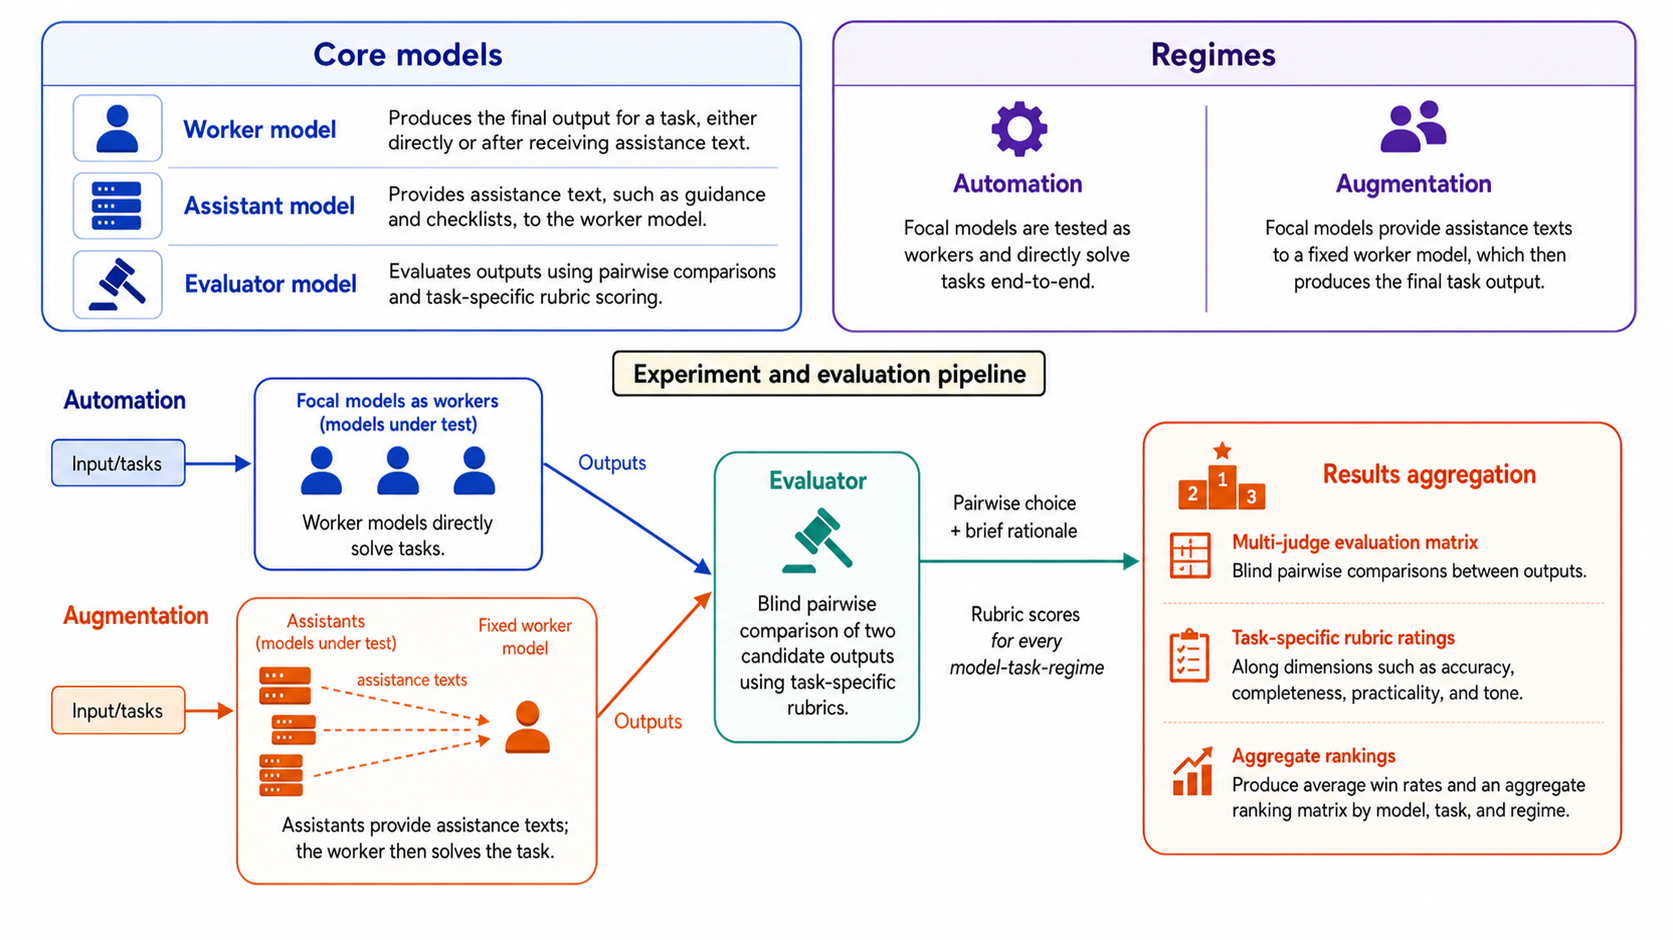
\includegraphics[width=\linewidth]{figures/methodology-final.png}
\caption{\textbf{Methodology pipeline.} The framework evaluates models in two usage modes: automation, where focal models directly solve tasks, and augmentation, where focal models provide an assistance text to a fixed worker model. Outputs are evaluated through rubric-guided pairwise comparisons and aggregated into model rankings by task and usage mode.}
\label{fig:methodology-pipeline}
\end{figure}


\subsection{Task Selection and Prompt Design}

We construct a benchmark of seven tasks representing activities commonly encountered in everyday and professional settings and associated with economically meaningful forms of work: counseling, market analysis, meal planning, operations research, tax preparation, travel planning, and tutoring. Tasks were chosen to vary in structure, domain knowledge, risk, and the degree to which human-facing judgment matters. Each task specifies an observable deliverable with concrete requirements, allowing evaluation to assess whether outputs satisfy stated constraints objectively rather than relying on subjective impressions of quality. Figure~\ref{fig:tasks} presents the full task set. The assistant model set and judge panel are reported in the supplementary document.

To make evaluation reliable, each task prompt is paired with a micro-rubric. The prompt specifies the required deliverable and the components that must be present. The rubric mirrors those components and scores each dimension on a 1--10 scale. Each task includes task-specific dimensions, such as dietary safety for meal planning or mathematical correctness for tutoring, as well as general dimensions such as instruction following, accuracy, practical usefulness, organization, and tone. We evaluate models pairwise to enable contrastive grading (which we found worked better), where the judge can compare models to determine winners rather than grade inherently subjective outputs. However, we also develop the task-specific rubrics to help ground the judge's decision, and also as a way for humans to reason about why certain outputs were judged better than others. 


\begin{figure}[htbp]
\centering
%
\includegraphics[width=\linewidth]{tasks.png}
\renewcommand{\arraystretch}{1.15}
\setlength{\tabcolsep}{6pt}
\small

\definecolor{planyellow}{RGB}{255,247,222}
\definecolor{profgreen}{RGB}{231,243,231}
\definecolor{humanpurple}{RGB}{237,236,250}
\definecolor{headnavy}{RGB}{16,42,94}

\begin{tabularx}{\linewidth}{
    >{\raggedright\arraybackslash\hsize=0.85\hsize}X
    >{\raggedright\arraybackslash\hsize=1.05\hsize}X
    >{\raggedright\arraybackslash\hsize=1.00\hsize}X
    >{\raggedright\arraybackslash\hsize=1.10\hsize}X}
\toprule
\rowcolor{headnavy}
\textcolor{white}{\textbf{Task}} &
\textcolor{white}{\textbf{Source}} &
\textcolor{white}{\textbf{Task type}} &
\textcolor{white}{\textbf{Deliverable}} \\
\midrule
\rowcolor{planyellow}
Menu Planning & GDPval & Structured planning & Seven-day constrained meal plan \\
\rowcolor{planyellow}
Travel Planning & GDPval & Structured planning & Tokyo itinerary under fixed budget \\
\rowcolor{profgreen}
Market Trends Analysis & GDPval & Professional / analytical & Client brief on natural gas trends \\
\rowcolor{profgreen}
Operations Research Analysis & Anthropic Economic Index & Professional / analytical & Executive logistics optimization memo \\
\rowcolor{profgreen}
Tax Preparation & Designed task & Professional / analytical & Tax discrepancy review and correction guidance \\
\rowcolor{humanpurple}
Counseling & Anthropic Economic Index & Human-facing interactive & Supportive counseling-style response \\
\rowcolor{humanpurple}
Tutoring Session Planning & Anthropic Economic Index & Human-facing interactive & Grade 3 lesson segment \\
\bottomrule
\end{tabularx}
\caption{\textbf{Tasks included in the benchmark.}
    The figure reports each task's source, broad task type, and required deliverable. Colors distinguish structured-planning tasks (yellow), professional or analytical tasks (green), and human-facing interactive tasks (purple). Tasks were drawn from GDPval and the Anthropic Economic Index, except for tax preparation, which was designed by the authors to provide a rule-based professional task with verifiable discrepancies. Full task prompts and evaluation rubrics are provided in the supplementary document.}
\label{fig:tasks}
\end{figure}


This alignment between prompt and rubric is central to the framework. We do not ask evaluators to make an undifferentiated and subjective judgment of quality. Instead, they judge whether the response satisfies observable dimensions of the task that are quantifiable and comparatively objective to assess. For example, the travel-planning rubric separately measures cost realism, itinerary quality, hotel and transportation practicality, and handling of uncertainty. Meanwhile, the tax-preparation rubric separately measures rule accuracy, discrepancy detection, calculation quality, form guidance, dependent analysis, and client-facing clarity. Figure~\ref{fig:prompt-rubric-design} summarizes the alignment between task prompts, task-specific micro-rubrics, general evaluation dimensions, and the augmentation assistance text constraint.

\begin{figure}[htbp]
\centering
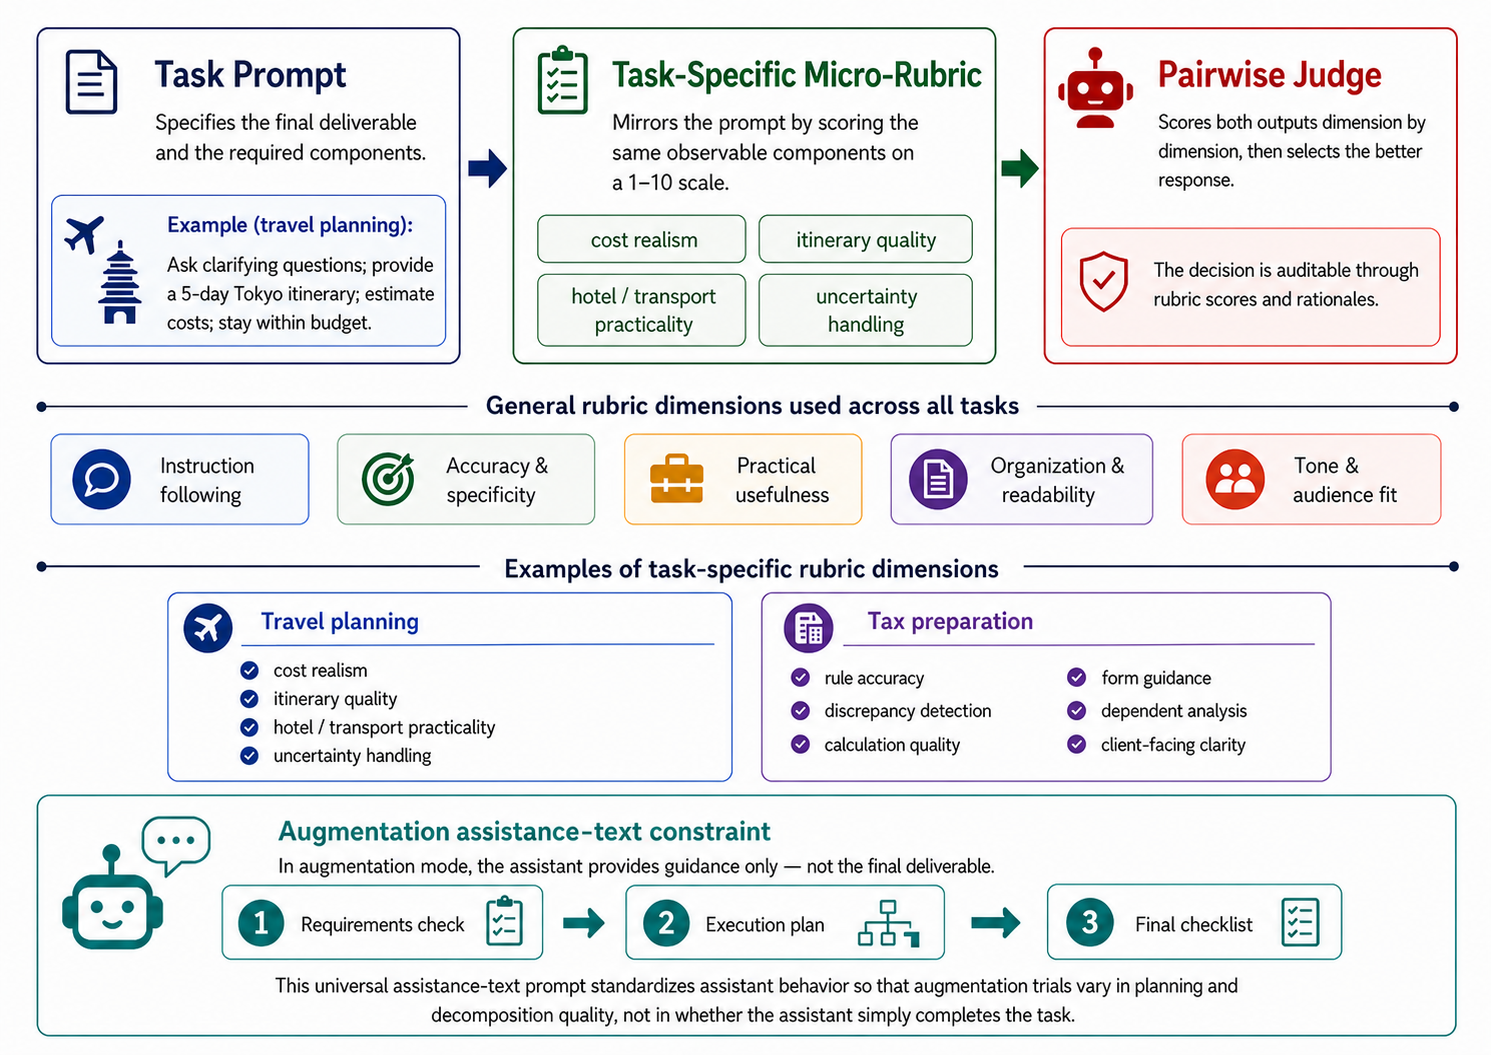
\includegraphics[width=\linewidth]{figures/evals-final.png}
\caption{\textbf{Prompt and rubric design.} Each task prompt specifies observable deliverable requirements, which are mirrored by task-specific micro-rubrics. General rubric dimensions are held constant across tasks, while task-specific dimensions vary by domain. In augmentation mode, the assistance text creation prompt constrains assistant models to provide process guidance rather than the final deliverable.}
\label{fig:prompt-rubric-design}
\end{figure}


Figure~\ref{fig:prompt-rubric-example} illustrates the prompt and rubrics for travel planning. Full prompts, assistance texts, and rubrics for all tasks appear in the supplementary document. In augmentation mode, each assistant model receives a universal assistance text creation prompt that instructs it to produce a process-oriented plan for the worker, rather than completing the task itself. The prompt specifies a three-phase structure: a requirements check, an execution plan, and a final checklist. It additionally constrains the assistant to provide guidance only, explicitly prohibiting production of the final deliverable. This design ensures that what varies across augmentation trials is the quality of the assistant's planning and decomposition, not whether the assistant simply solved the task on the worker's behalf. 


\begin{figure}[htbp]
\centering
\footnotesize

\definecolor{taskblue}{RGB}{220,235,252}
\definecolor{taskblueframe}{RGB}{16,42,94}
\definecolor{rubricmint}{RGB}{225,245,225}
\definecolor{rubricmintframe}{RGB}{16,42,94}
\definecolor{assistpeach}{RGB}{255,242,218}
\definecolor{assistpeachframe}{RGB}{16,42,94}


\scalebox{0.95}{%
\begin{minipage}{\linewidth}
\begin{tcolorbox}[taskprompt, enhanced, colback=taskblue, colframe=taskblueframe, colbacktitle=taskblueframe, coltitle=white, title=Task Prompt --- Travel Planning]
Create a 5-day Tokyo itinerary for one traveler next month with a total budget of \$2,500 USD, excluding passport costs. The traveler is departing from San Francisco. Clearly state assumptions and give clarifying questions before the provisional plan. Use realistic estimates, label them as estimates, and keep the plan budget-aware.
\end{tcolorbox}

\vspace{0.4em}

\begin{tcolorbox}[rubricbox, enhanced, colback=rubricmint, colframe=rubricmintframe, colbacktitle=rubricmintframe, coltitle=white, title=Evaluation Rubric --- Travel Planning]
Score each dimension from 1 (lowest) to 10 (highest):
\begin{enumerate}
  \setlength{\itemsep}{0pt}
  \item Completeness: covers questions, costs, hotels, transport, customs/regulations, itinerary, and budget confirmation.
  \item Cost realism and arithmetic: flights, lodging, transport, food/activities, and total are plausible and correctly summed. Penalize outputs that exceed the budget.
  \item Hotel and transport practicality: viable hotel options, airport/transit guidance, rail/pass advice.
  \item Itinerary quality: 5 days with morning/afternoon/evening plans that are geographically sensible and well-optimized for distance and fatigue.
  \item Travel-agent professionalism: clear, customer-focused, with appropriate caveats around estimates.
  \item Handling uncertainty: asks clarifying questions for missing information while still providing a useful provisional plan.
\end{enumerate}
\end{tcolorbox}
\end{minipage}}

\vspace{0.4em}

\scalebox{0.95}{%
\begin{minipage}{\linewidth}
\begin{tcolorbox}[taskprompt, enhanced, fonttitle=\bfseries, colback=assistpeach, colframe=assistpeachframe, colbacktitle=assistpeachframe, coltitle=white, title=Assistance Text Creation Prompt --- Universal (Abridged)]
Produce a 200--250 word, process-focused assistance text without writing the final deliverable.

Organize the assistance text into three phases:
\begin{enumerate}
    \setlength{\itemsep}{1pt}
    \item \textbf{Requirements Check:} identify the deliverable, audience, tone, constraints, and required components.
    \item \textbf{Plan and Structure:} recommend a general response structure and explain how to balance completeness, clarity, and tone.
    \item \textbf{Self-Review and Finalize:} provide a concise checklist for reviewing the response before submission.
\end{enumerate}

Do not solve the task, provide task-specific content or examples, or write sentences that could be copied into the final answer. Keep the guidance process-focused.

\medskip
\textit{Abridged for presentation. The full verbatim experimental prompt is provided in the supplementary document.}
\end{tcolorbox}
\end{minipage}}

\caption{\textbf{Illustrative task prompt, evaluation rubric, and assistance-text
instruction.} The travel-planning example shows how observable task requirements (top) map onto task-specific rubric dimensions (middle). In augmentation mode, the assistant additionally receives the universal assistance text creation prompt shown above (bottom), which requires process-oriented guidance while prohibiting completion of the final deliverable. The complete prompts and rubrics are provided in the supplementary document.}
\label{fig:prompt-rubric-example}
\end{figure}


Augmentation can be operationalized in many ways, ranging from an assistant that drafts content for the worker to edit, to one that supplies worked examples or directly corrects worker errors. Education research draws a similar distinction: procedural, strategic, and metagonitive scaffolding that shapes \emph{how} a learner approaches a task, versus conceptual scaffolding that supplies domain content \citep{hannafin1999}. We study process-oriented scaffolding, in which the assistant shapes how the worker approaches the task but never supplies solution content. This mirrors the educational ideal of teaching a learner to perform a task rather than performing it for them \citep{wood1976, vandepol2010} and isolates the value of guidance from the assistant's own task-solving ability. By design, it is a deliberately conservative form of assistance and lower bound on what augmentation can achieve, since it withholds conceptual, content-bearing support. Thus, the results should be read as characterizing this form rather than augmentation at large. However, the same fixed-worker methodology extends directly to richer forms of assistance, and mapping how augmentation value varies across richer types is a natural next steps our framework is designed to support. The full assistance prompt is provided in the supplementary document.

\subsection{Evaluation Procedure}

\begin{figure}[htbp]
\centering
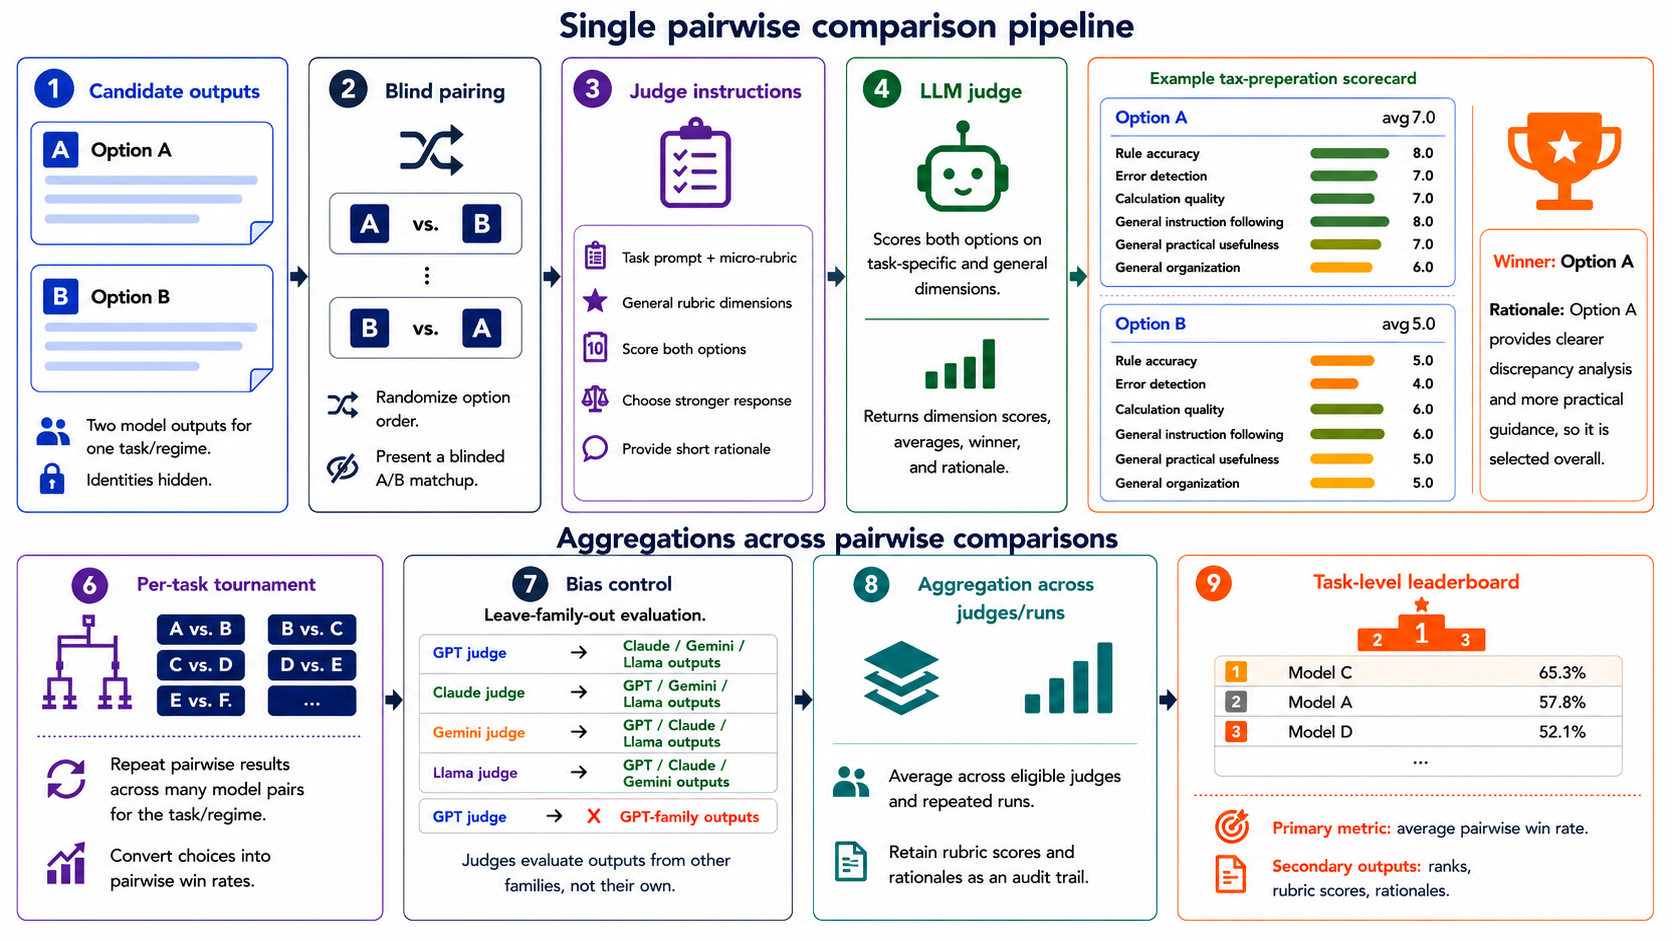
\includegraphics[width=\linewidth]{figures/eval-pipeline.png}
\caption{\textbf{Rubric-guided pairwise evaluation pipeline.} Candidate outputs are anonymized, randomly paired, and evaluated by LLM judges using task-specific and general rubric dimensions. Pairwise choices are converted into win rates, aggregated across eligible judges and repeated runs, and reported alongside rubric scores and rationales as an audit trail.}
\label{fig:eval-pipeline}
\end{figure}

% Following prior work on LLM-as-judge evaluation \citep{zheng2023} and pairwise preference benchmarking \citep{chiang2024}, we evaluate final outputs using blind pairwise comparisons conducted by a panel of LLM judges. Prior research finds that LLM judgments can achieve substantial agreement with human preferences when model identities are concealed and evaluators receive explicit criteria. Figure~\ref{fig:eval-pipeline} summarizes our evaluation pipeline.

Following prior work on LLM-as-judge evaluation and pairwise preference benchmarking \citep{zheng2023,chiang2024}, we evaluate final outputs through blind pairwise comparisons conducted by a panel of four LLM judges. Figure~\ref{fig:eval-pipeline} summarizes the procedure.

%Within each task and each usage mode, we run a complete round-robin over the ten models, scored by a panel of four LLM judges across ten independent runs, with each judge excluded from comparisons involving its own model family (assistant models and judge panel in Appendix~\ref{app:models}). In augmentation, the candidate pool also includes a \emph{plain} baseline—the fixed worker model with no assistance from external models—as a reference point for whether the assistant model helps at all. For each task and regime, candidate outputs are paired against one another, with model identities hidden from the evaluator and option order randomized. The evaluator scores both options explicitly across the task-specific and general rubric dimensions, averages the scores across all dimensions, and then selects the stronger response overall. To increase transparency, we also prompt the evaluator to provide a short rationale supporting their choice. Pairwise comparisons are conducted within a regime; automation and augmentation outputs are never judged against each other directly. Cross-mode comparison is made at the level of ranks, not raw pairwise outcomes. Across non-tied comparisons, judges' final choices agree with the option receiving the higher average rubric score in 99.7\% of cases, indicating that pairwise outcomes are directionally consistent with the underlying dimension-level evaluations rather than arbitrary preferences (Appendix~\ref{app:llm-judge-validity}). 

For each task, usage mode, and independent run, we conduct a complete round-robin tournament among the ten candidate outputs. In augmentation, this candidate set includes the \emph{plain} baseline: the fixed worker operating without an assistance text. This baseline indicates whether receiving assistance improves the worker's output at all. Automation and augmentation
outputs are evaluated in separate tournaments and are never compared directly. 

For every comparison, model identities are concealed and option order is randomized. The judge scores both responses from 1 to 10 on the task-specific and general rubric dimensions, computes an average score for each response, selects the stronger response, and provides a short rationale. We apply \emph{leave-family-out} evaluation: a judge does not evaluate comparisons containing outputs from its own model family. The model and judge panels are reported in the supplementary document.

We treat pairwise comparison and rubric-based scoring as complementary components of our evaluation pipeline. Pairwise judgments provide the primary ranking signal because relative comparisons can recover expert-intended quality orderings more reliably and with lower annotation time than absolute rubric scores in judgment-intensive professional tasks \citep{yang2026judgmentbench}. More broadly, rubric-guided pairwise LLM judgments have been shown to align closely with human preferences \citep{zheng2023}. Pairwise choices alone, however, reveal which response is preferred without fully explaining why. Dimension-level rubric scores provide an inspectable diagnostic record, identifying the specific strengths and weaknesses underlying each comparison and supporting our qualitative analysis. Because rubric-based evaluation is itself sensitive to score calibration, scale use, and score-option ordering \citep{xu2026pointwisepairwise}, we use standardized rubric-derived rankings as a robustness check rather than as a replacement for pairwise comparison. We therefore use pairwise outcomes to construct the primary rankings and standardized rubric scores to interpret those rankings and test their robustness. Together, the two signals make the evaluation more reliable, transparent, and diagnostically useful. Across non-tied comparisons, the selected response receives the higher mean rubric score in 99.7\% of cases. In addition to the consistency between a judge's choice and its own rubric scores, we also measure agreement across judges. We separately assess inter-judge
reliability across all runs. Across 6,265 comparisons evaluated by at least two eligible judges, the judges select the same winner in 71.0\% of cases. Agreement is higher in automation (74.5\%) than in augmentation (67.8\%). The supplementary document reports the full LLM-judge reliability analysis.

\begin{figure}[htbp]
\centering
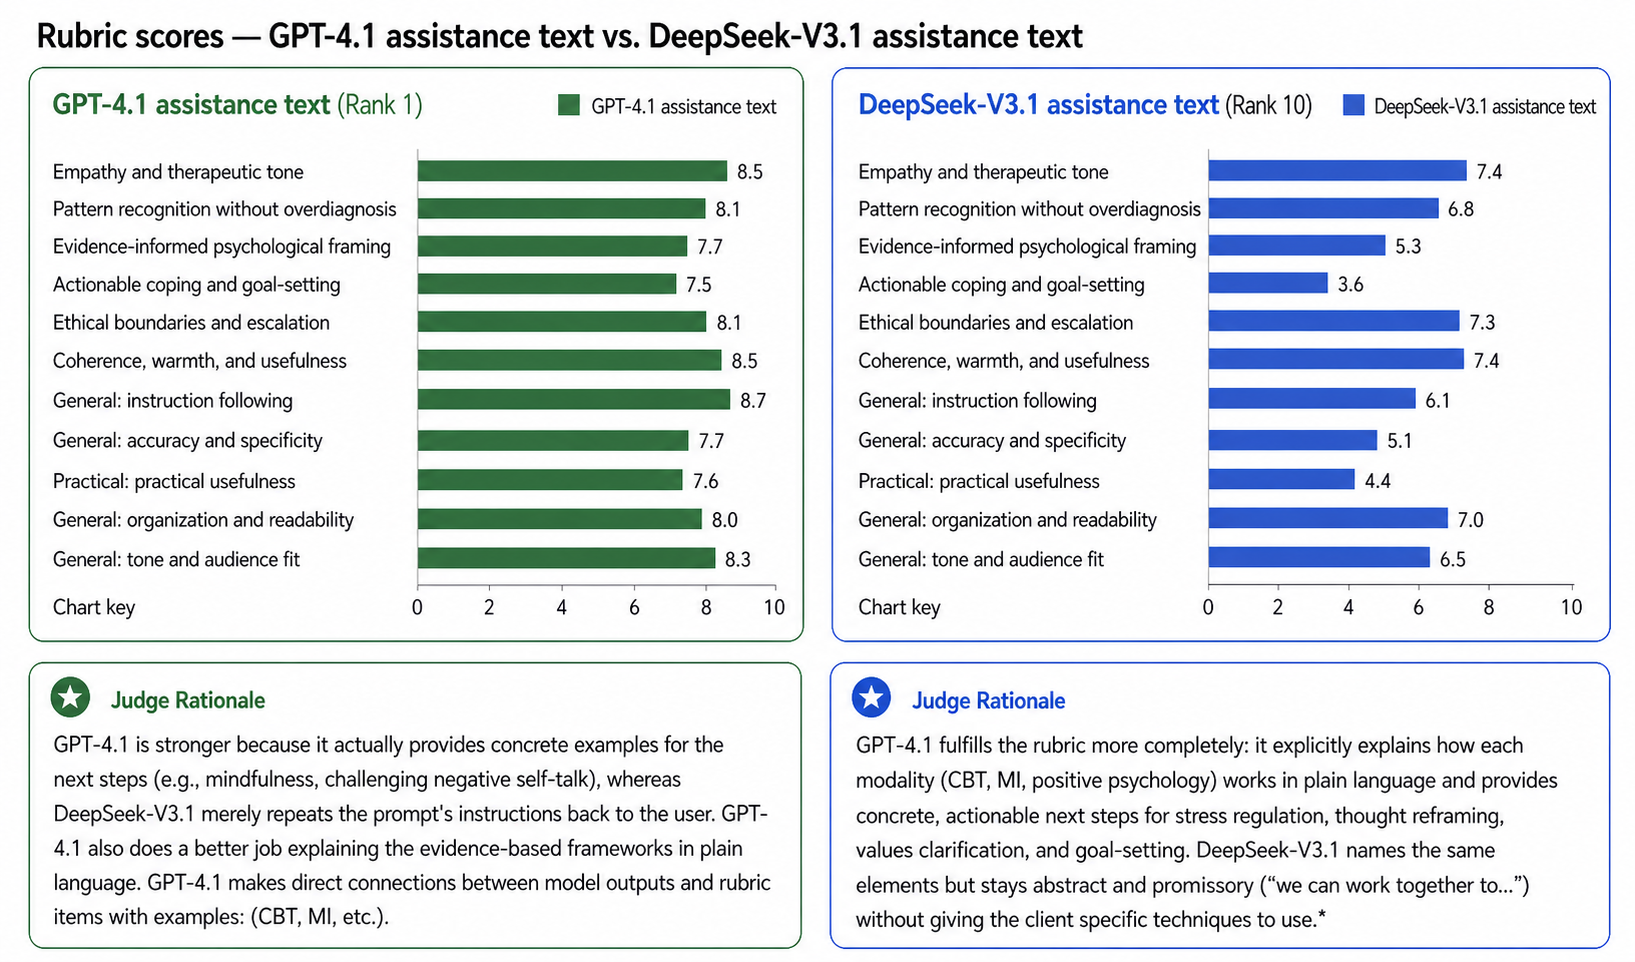
\includegraphics[width=0.87\linewidth]{figures/eval-example.png}
\caption{\textbf{Rubric-guided scoring.} Judge rationales explain the pairwise choice made. The models used in this example are GPT-4.1 and DeepSeek-V3.1 in augmentation mode for the counseling task. The corresponding outputs are in the supplementary document.}
\label{fig:eval-example}
\end{figure}

We aggregate the evaluations in three stages. First, each judge's choices are converted into a pairwise win rate for every model within each task and usage mode.
Second, models are ranked by win rate, and their ranks are averaged across eligible judges and ten independent runs. Third, task-level ranks are combined through a rank-of-ranks aggregation to obtain an overall ordering for each usage mode. We retain all task-level rankings, rubric scores, and rationales for subsequent analysis.

Figure~\ref{fig:eval-example} illustrates the resulting audit trail using two counseling outputs from augmentation mode. It reports the dimension-level
scores and judge rationale for outputs produced with assistance texts from GPT-4.1 and DeepSeek-V3.1. The corresponding assistance texts and final worker
outputs appear in the supplementary document.

% An example is provided in Figure~\ref{fig:eval-example}. It shows the rubric-specific scores for outputs assisted by GPT-4.1 (ranked overall best) and assisted by DeepSeek-V3.1 (ranked overall worst) for the counseling task in the first run. The LLM judge rationale is also included at the bottom of the figure. To see the output for each augmenter, please refer to Appendix~\ref{app:eval-examples}.

% Our ranking pipeline proceeds in four steps. First, for each task and regime, every candidate output is compared pairwise against every other candidate, with model identities hidden and option order randomized. Second, each eligible judge's pairwise choices are converted into a per-model win rate. Third, within each task and regime, models are ordered by average win rate to produce a per-judge ranking, which we average across eligible judges (under leave-one-family-out masking) and across runs. Fourth, we combine these task-level average ranks into a single ordering per regime using a rank-of-ranks aggregation, while retaining the task-level rankings used throughout our analyses.

    
\section{Results}

    
We report two sets of results. First, we examine the \emph{automation} mode, where each model solves the task directly. It is imperative to acknowledge here that these results characterize models' performance on single-turn, bounded professional deliverables completed \emph{without} tool usages. This setting differs from public agentic benchmarks, which often evaluate multi-step tool use, planning, and interaction with external environments; model orderings from those benchmarks therefore need not transfer to the setting studied here.

Second, we examine the \emph{augmentation} mode, where each assistant model acts as a coach that supplies a process guidance to a fixed GPT-3.5-Turbo worker that produces the final output, rather than solving the task itself. We then compare augmentation rankings to automation rankings to test whether strong direct task-solving ability also implies strong assistant ability. Across both analyses, rankings are computed over ten independent runs of the full pipeline. Main-text figures report within-task \emph{rank of ranks} (integer ranks derived from mean ranks across runs); the supplementary document reports mean rank with standard error ($\mathrm{SE}=\mathrm{SD}/\sqrt{10}$). All rankings are computed over the full candidate pool, which includes the unaided GPT-3.5-Turbo baseline. The accompanying supplementary materials provide the detailed audit trail for readers who wish to inspect individual tasks, models, and judgments.

Our central result is that model performance is both task-specific and mode-specific. In automation, rankings are concentrated around a small set of strong direct solvers, although this ordering should be interpreted as specific to
the bounded, single-turn tasks evaluated here rather than as a universal ranking of model capability. In augmentation, no single assistant model dominates across all tasks: different task domains reward different assistant behaviors, and several tasks are best handled by the unaided worker baseline rather than by an external assistance. This divergence suggests that standard automation benchmarks do not capture an economically important capability, whether a model can improve another worker's output through planning and decomposition. We use the paper figures to summarize the main patterns; the interactive dashboard provides a more detailed audit trail for readers who wish to inspect individual tasks, models, and judgments.

\subsection{Model Rankings in Automation Mode}

\begin{figure}[htbp]
    \centering
    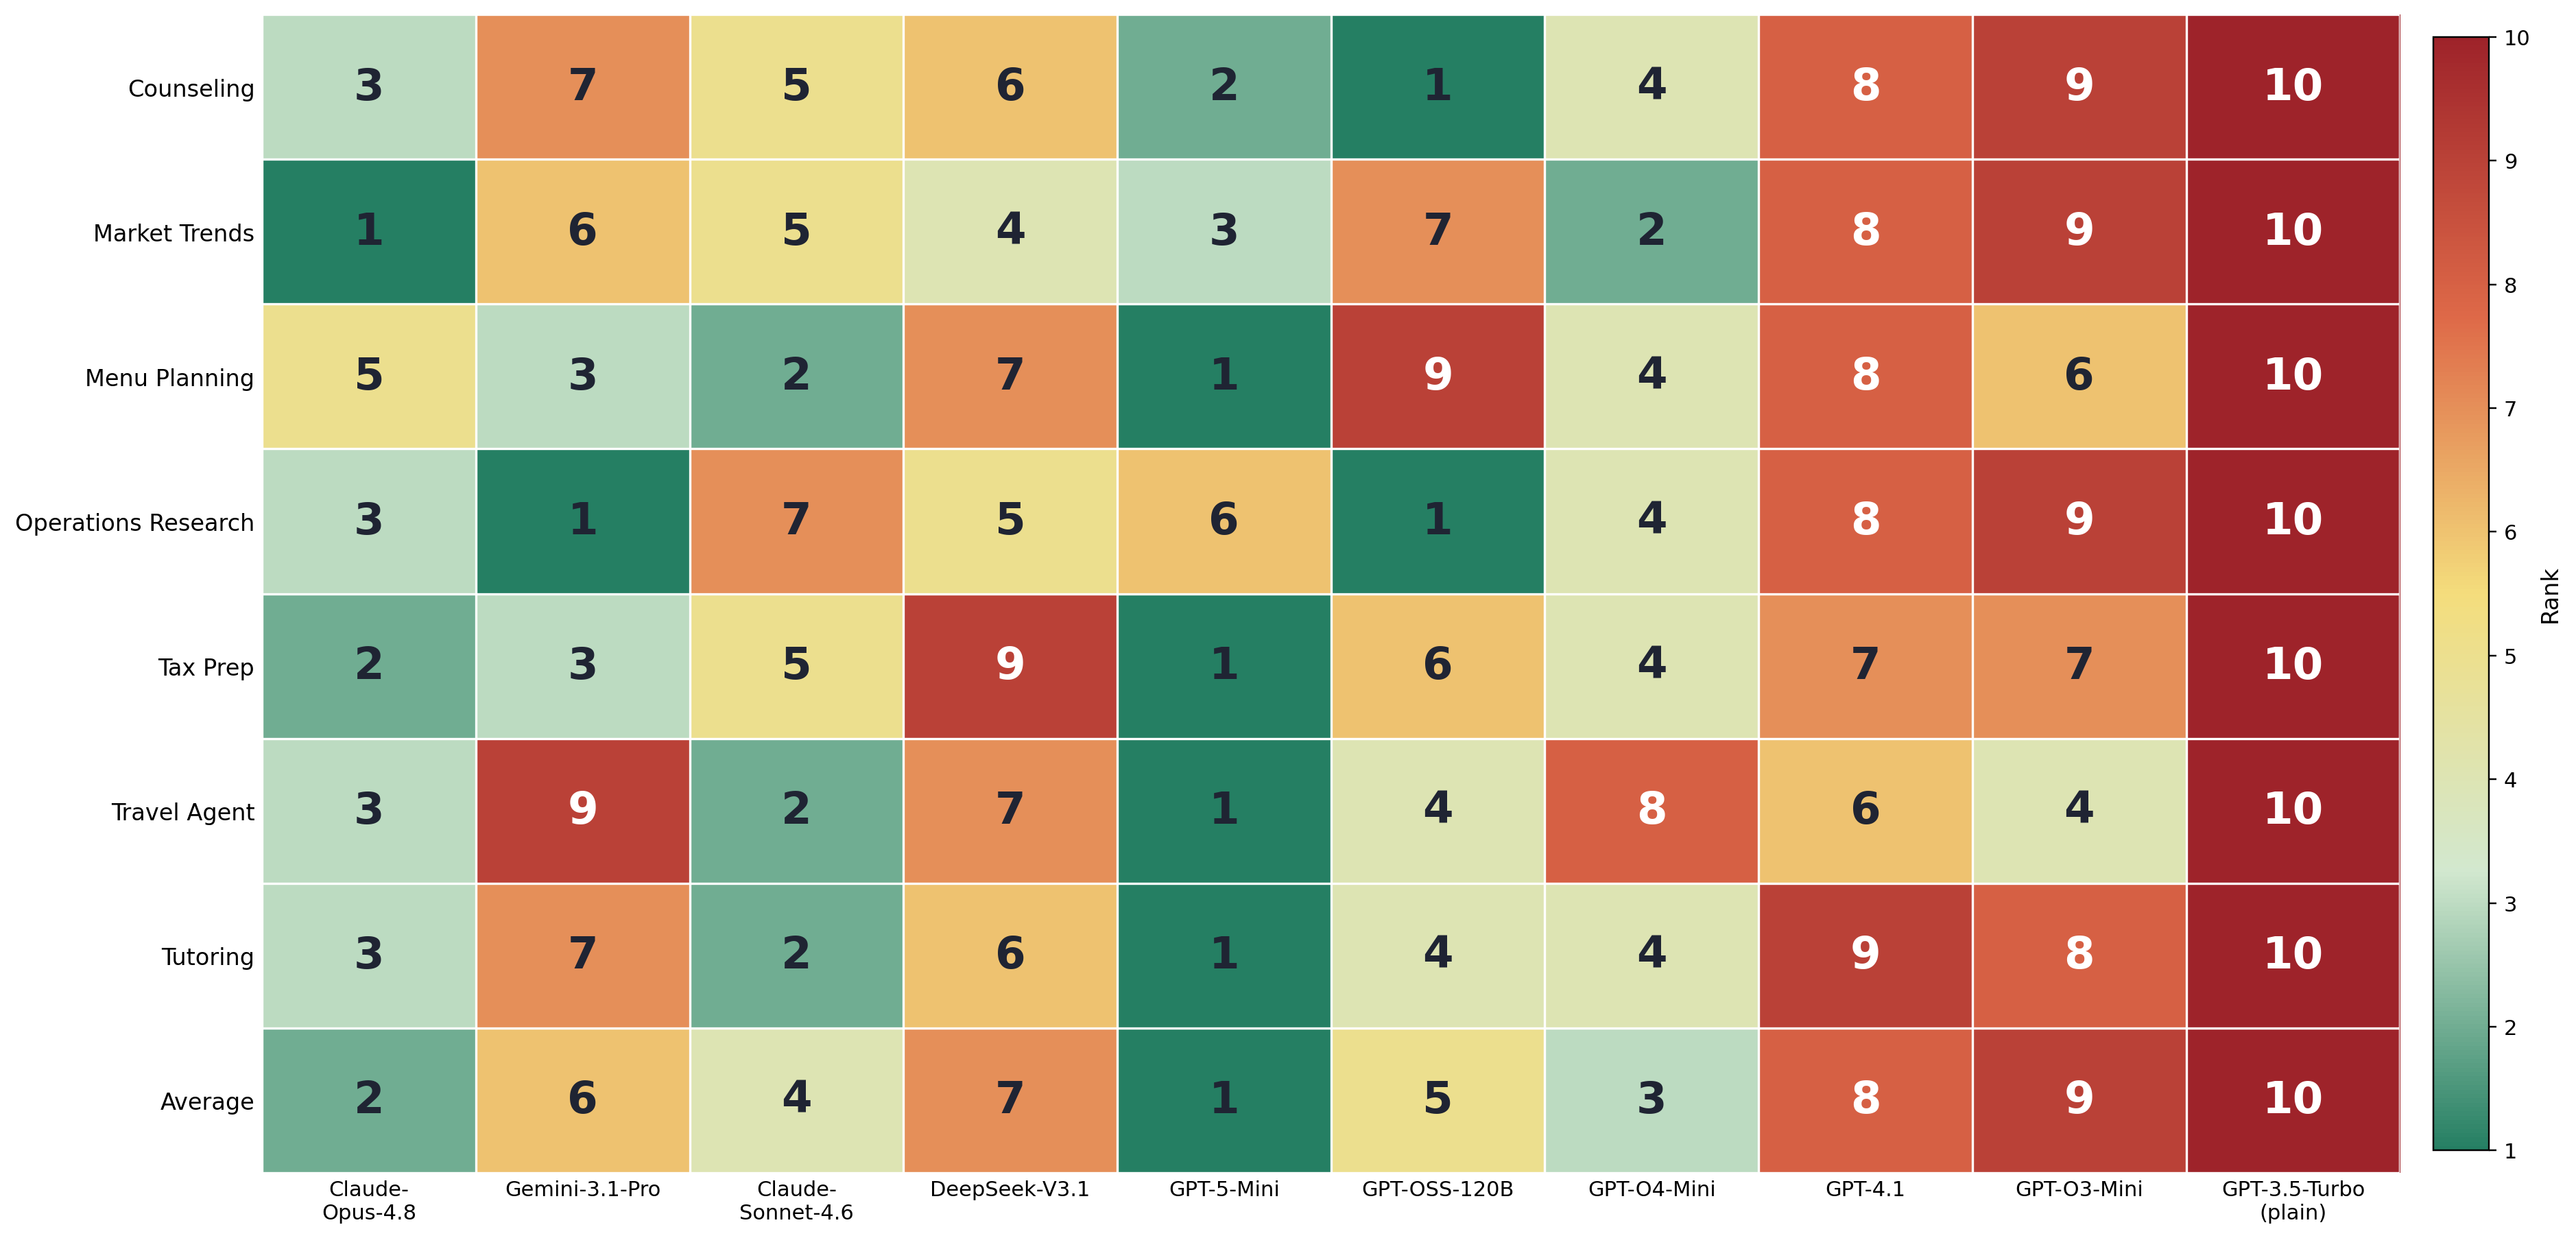
\includegraphics[width=\linewidth]{figures/figure2a_automation_heatmap.png}
    \caption{\textbf{Automation rankings by task, averaged across ten independent runs.} For each task, we first average each model's within-run rank across the ten runs and then rank these mean values to produce the displayed rank of ranks (1 = best). Rankings are computed using unrounded mean ranks. Exact ties receive the same rank, with the subsequent rank skipped (e.g., 1, 1, 3). Models are ordered from newest to oldest from left to right. Lower ranks indicate better performance. Mean ranks and standard errors are reported in the supplementary document.}
    \label{fig:automation-heatmap}
\end{figure}
% change model capability language
% In automation, rankings are directionally aligned with conventional capability rankings. Stronger frontier models tend to perform better as direct task solvers, while weaker or older models fall toward the bottom. Figure~\ref{fig:automation-heatmap} reports these rankings by task. GPT-5-Mini has the best average rank across tasks, followed by Claude-Opus-4.8. GPT-O4-Mini and Claude-Sonnet-4.6 form the next tier, while GPT-3.5-Turbo (plain) ranks last on average, as expected for a low-cost baseline. This is reassuring before we turn to augmentation, as stronger direct solvers are recognized as such across most task domains.

Figure~\ref{fig:automation-heatmap} reports model rankings in the automation mode by task across ten independent runs. GPT-5-Mini has the best average rank across tasks, followed by Claude-Opus-4.8. GPT-O4-Mini and Claude-Sonnet-4.6 form the next tier, while GPT-3.5-Turbo (plain) ranks last on average. The task-level results are also relatively concentrated. GPT-5-Mini ranks first in menu planning, tax preparation, travel planning, and tutoring; Claude-Opus-4.8 ranks first in market-trends analysis; GPT-OSS-120B ranks first in counseling; and GPT-OSS-120B and Gemini-3.1-Pro jointly lead operations research. 

The automation results characterize direct task performance under the particular roles, tasks, and interaction constraints studied here. Automation places the full burden of task completion on the model. It must interpret the prompt, track constraints, produce the final deliverable, and avoid errors without help from another system, so general model capability matters more. We next examine whether these same models retain their relative advantages when they instead assist a fixed downstream worker.
%The task-level pattern is also concentrated. GPT-5-Mini ranks first in menu planning, tax preparation, travel planning, and tutoring. Claude-Opus-4.8 ranks first in market-trends analysis, GPT-OSS-120B ranks first in counseling, along with Gemini-3.1-Pro jointly leading in operations research. A likely reason automation tracks conventional capability more closely is that it places the full burden of task completion on the  model. It must interpret the prompt, track constraints, produce the final deliverable, and avoid errors without help from another system, so general model capability matters more. Augmentation, by contrast, tests whether a model can improve a fixed worker's output through guidance; this depends not only on raw task-solving ability but on whether the guidance is usable by the worker. We examine that regime next.

\subsection{Model Rankings in Augmentation Mode}

\begin{figure}[htbp]
    \centering
    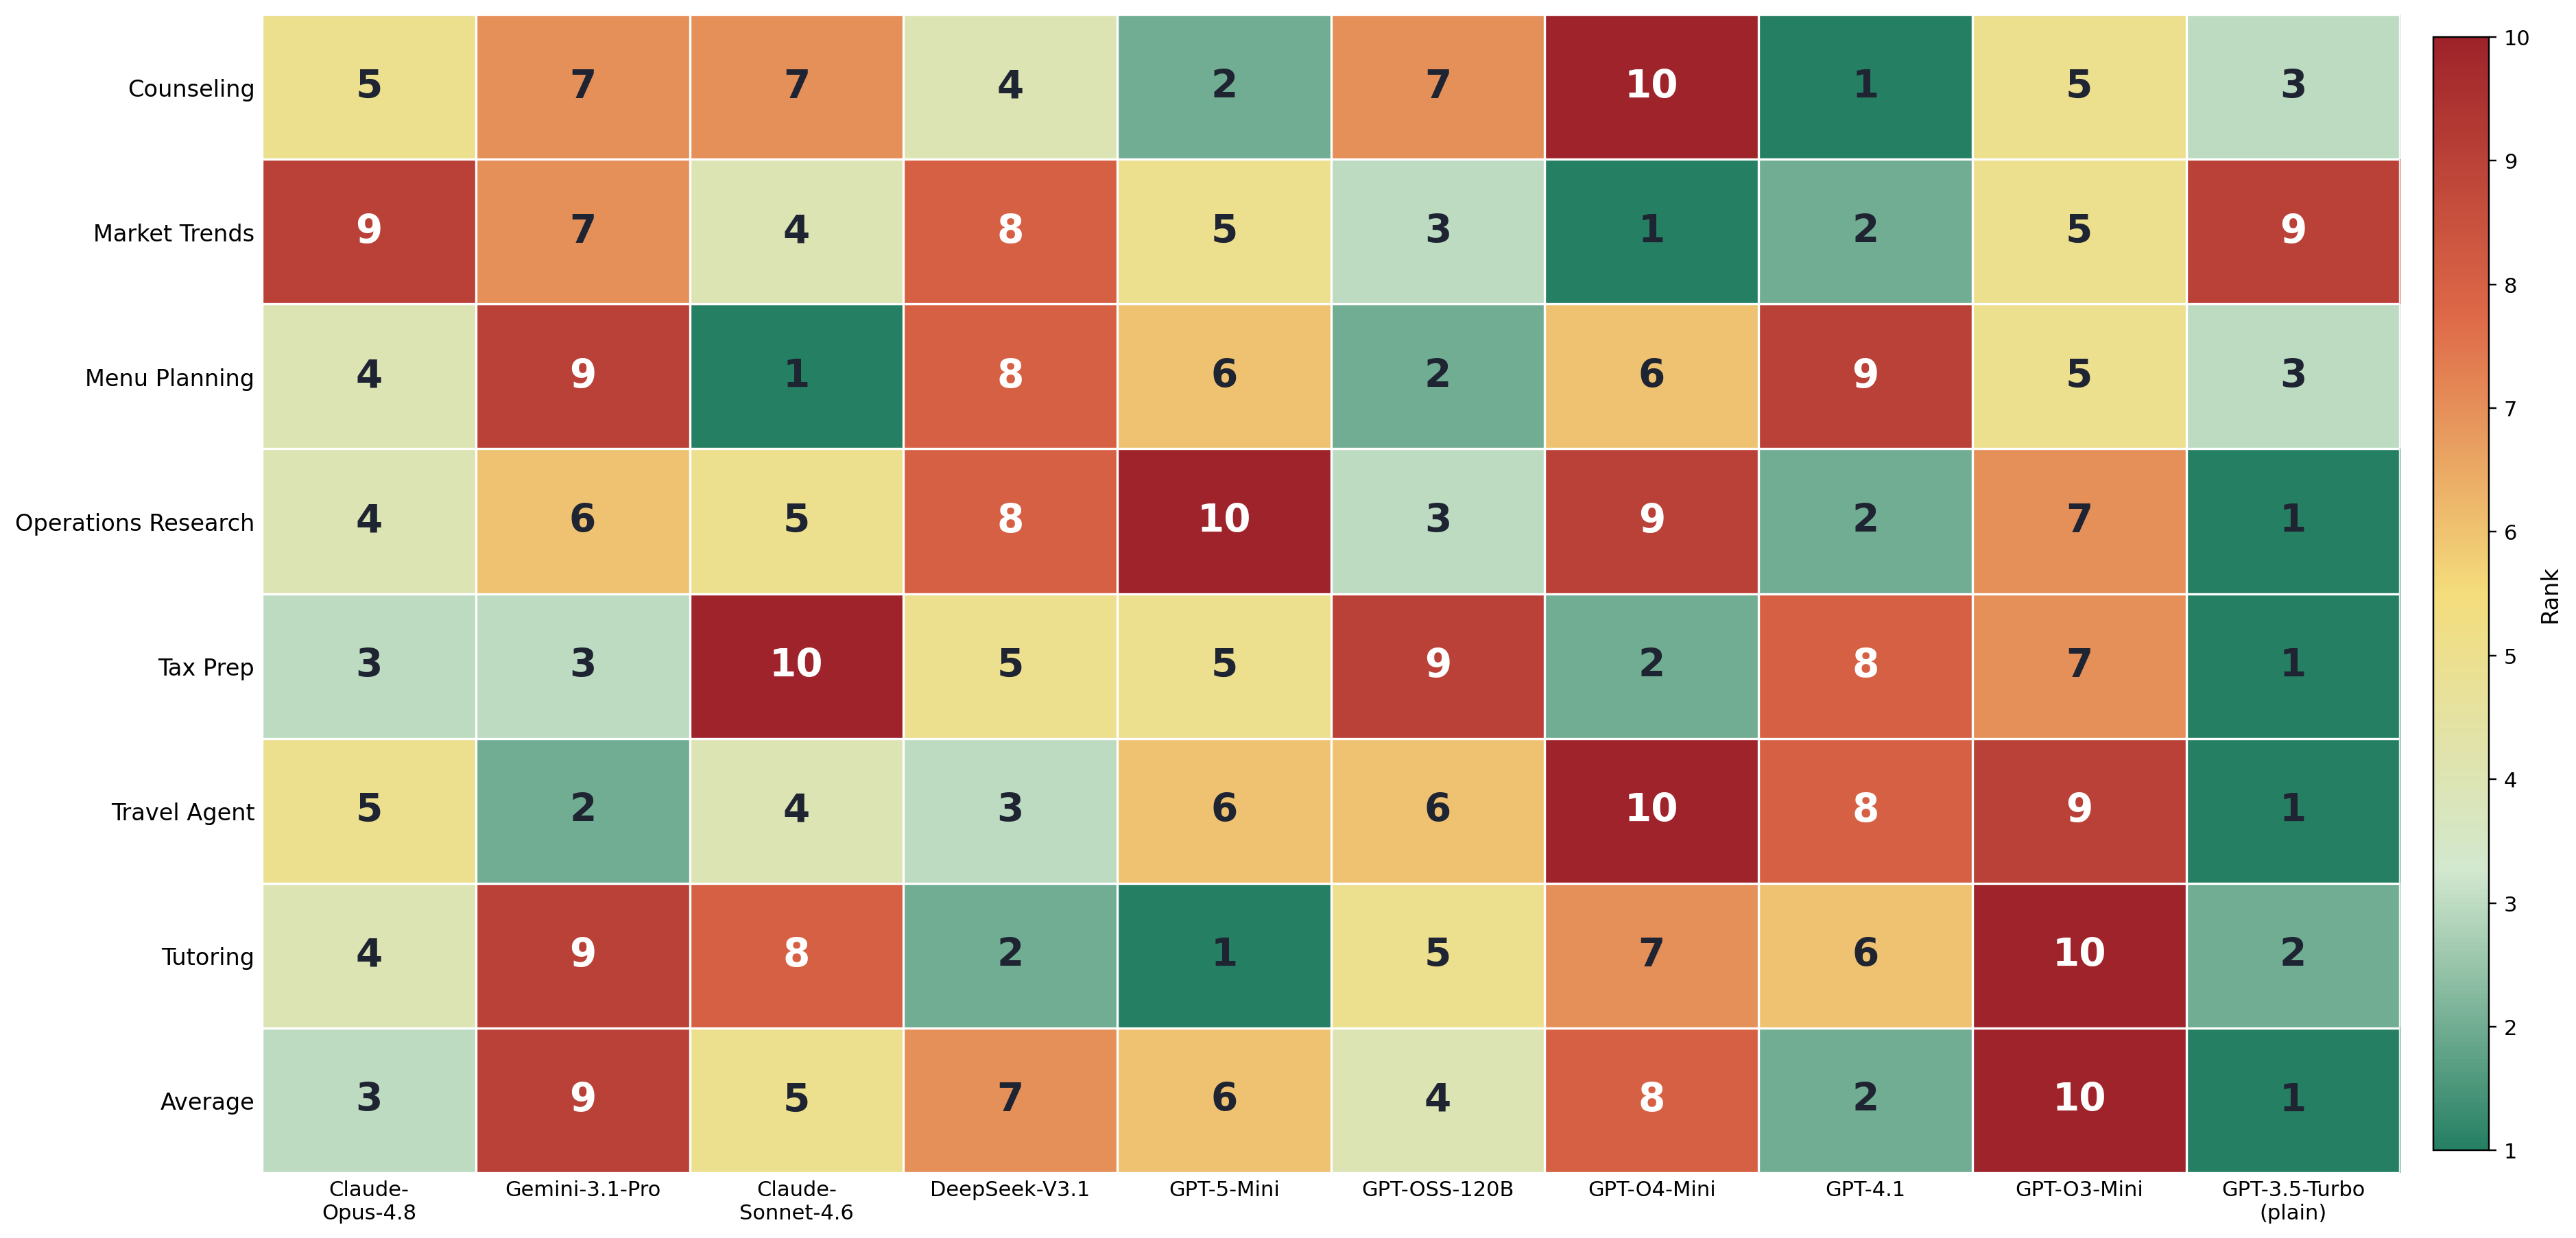
\includegraphics[width=\linewidth]{figures/figure1_augmentation_heatmap.png}
    \caption{\textbf{Augmentation rankings by task, averaged across ten independent runs.} For each task, we first average each model's within-run rank across the ten runs and then rank these mean values to produce the displayed rank of ranks (1 = best). Rankings are computed using unrounded mean ranks. Exact ties receive the same rank, with the subsequent rank skipped (e.g., 1, 1, 3). Models are ordered from newest to oldest from left to right, with GPT-3.5-Turbo (plain), the unaided worker baseline, shown at far right. Lower ranks indicate better performance. Mean ranks and standard errors are reported in the supplementary document.}
    \label{fig:augmentation-heatmap}
\end{figure}

Figure~\ref{fig:augmentation-heatmap} reports model rankings in the augmentation mode across ten independent runs. Each assistant model provides a process guidance in a form of an assistance text to a fixed GPT-3.5-Turbo worker, which then produces the final task output. The figure shows substantial heterogeneity across tasks: no single assistant model consistently ranks first across the task set, and the relative ordering of models shifts across counseling, tutoring, planning, and analytical tasks.

Unlike automation, the best assistant changes substantially across tasks in augmentation. GPT-4.1 ranks first in counseling, GPT-O4-Mini in market-trends analysis, GPT-5-Mini in menu planning and tutoring. However, the unaided GPT-3.5-Turbo worker baseline ranks first in operations research, tax preparation, and travel planning when it is included in the full candidate pool. The best-performing assistant therefore differs by domain rather than converging on a single model, and in some tasks assistant guidance does not improve on the fixed worker's unaided output, even worsening it.

The pattern also differs by task type. Among the assistant models, GPT-4.1 performs especially well in counseling, consistent with strength in professionally framed guidance and sensitive response structure. GPT-O4-Mini leads in market-trends analysis, where the rubric rewards concise synthesis, specificity, and actionable interpretation. GPT-5-Mini leads in menu planning and tutoring and is the best assistant in tax preparation, suggesting strength on tasks that require constraint tracking, complete deliverables, and structured explanation. GPT-OSS-120B leads among assistants in operations research, where the rubric rewards optimization framing and trade-off reasoning. Claude-Sonnet-4.6 leads among assistants in travel planning, where practical sequencing, budget awareness, and itinerary usability are central. These results suggest that different models provide different kinds of useful guidance, but the mechanisms require qualitative analysis of the guidance and the resulting worker outputs, which we return to in Section~\ref{sec:analysis}.

Importantly, these ranking differences are unlikely to be driven by models excelling on one general evaluation dimension but not another. Across the five general rubric dimensions (instruction following, accuracy and specificity, practical usefulness, organization and readability, and tone/audience fit), most models receive similar relative scores on each dimension rather than specializing on a single axis; the supplementary document reports the corresponding profiles. Augmentation rankings therefore reflect differences in overall assistant quality and task fit rather than artifacts of how the general rubric is weighted. Models do not win because they are disproportionately strong on, say, organization but weak on accuracy. The task-specific pairwise outcomes point to genuine differences in how each model guides the fixed worker.

\subsection{Automation Rankings Differ From Augmentation Rankings}
\label{sec:role-swap}

To quantify the relationship between the two usage modes, let
$r^{(k)}_{mts}$ denote the within-task rank of assistant model $m$ on task
$t$, in usage mode $s\in\{\mathrm{auto},\mathrm{aug}\}$, and independent run
$k\in\{1,\ldots,10\}$, where lower values indicate better performance. We
first average over runs,
\begin{equation}
    \bar r_{mts}=\frac{1}{10}\sum_{k=1}^{10}r^{(k)}_{mts}.
\end{equation}
For each task, we then compute
\begin{equation}
    \rho_t=\operatorname{corr}_{\mathrm{S}}
    \!\left(
      \{\bar r_{mt,\mathrm{auto}}\}_{m\in\mathcal{M}},
      \{\bar r_{mt,\mathrm{aug}}\}_{m\in\mathcal{M}}
    \right),
    \label{eq:task-mode-correlation}
\end{equation}
where $\operatorname{corr}_{\mathrm{S}}$ is Spearman's rank correlation and $\mathcal{M}$ contains the nine assistant models evaluated in both usage modes. The unaided worker is excluded because it has no corresponding assistant model in automation. For the model-level comparison, we additionally average
$\bar r_{mts}$ over the seven tasks before computing the same correlation in each usage mode. Because reverse rank is a monotonic transformation of rank, it produces the same Spearman correlations.

\begin{figure}[htbp]
    \centering
    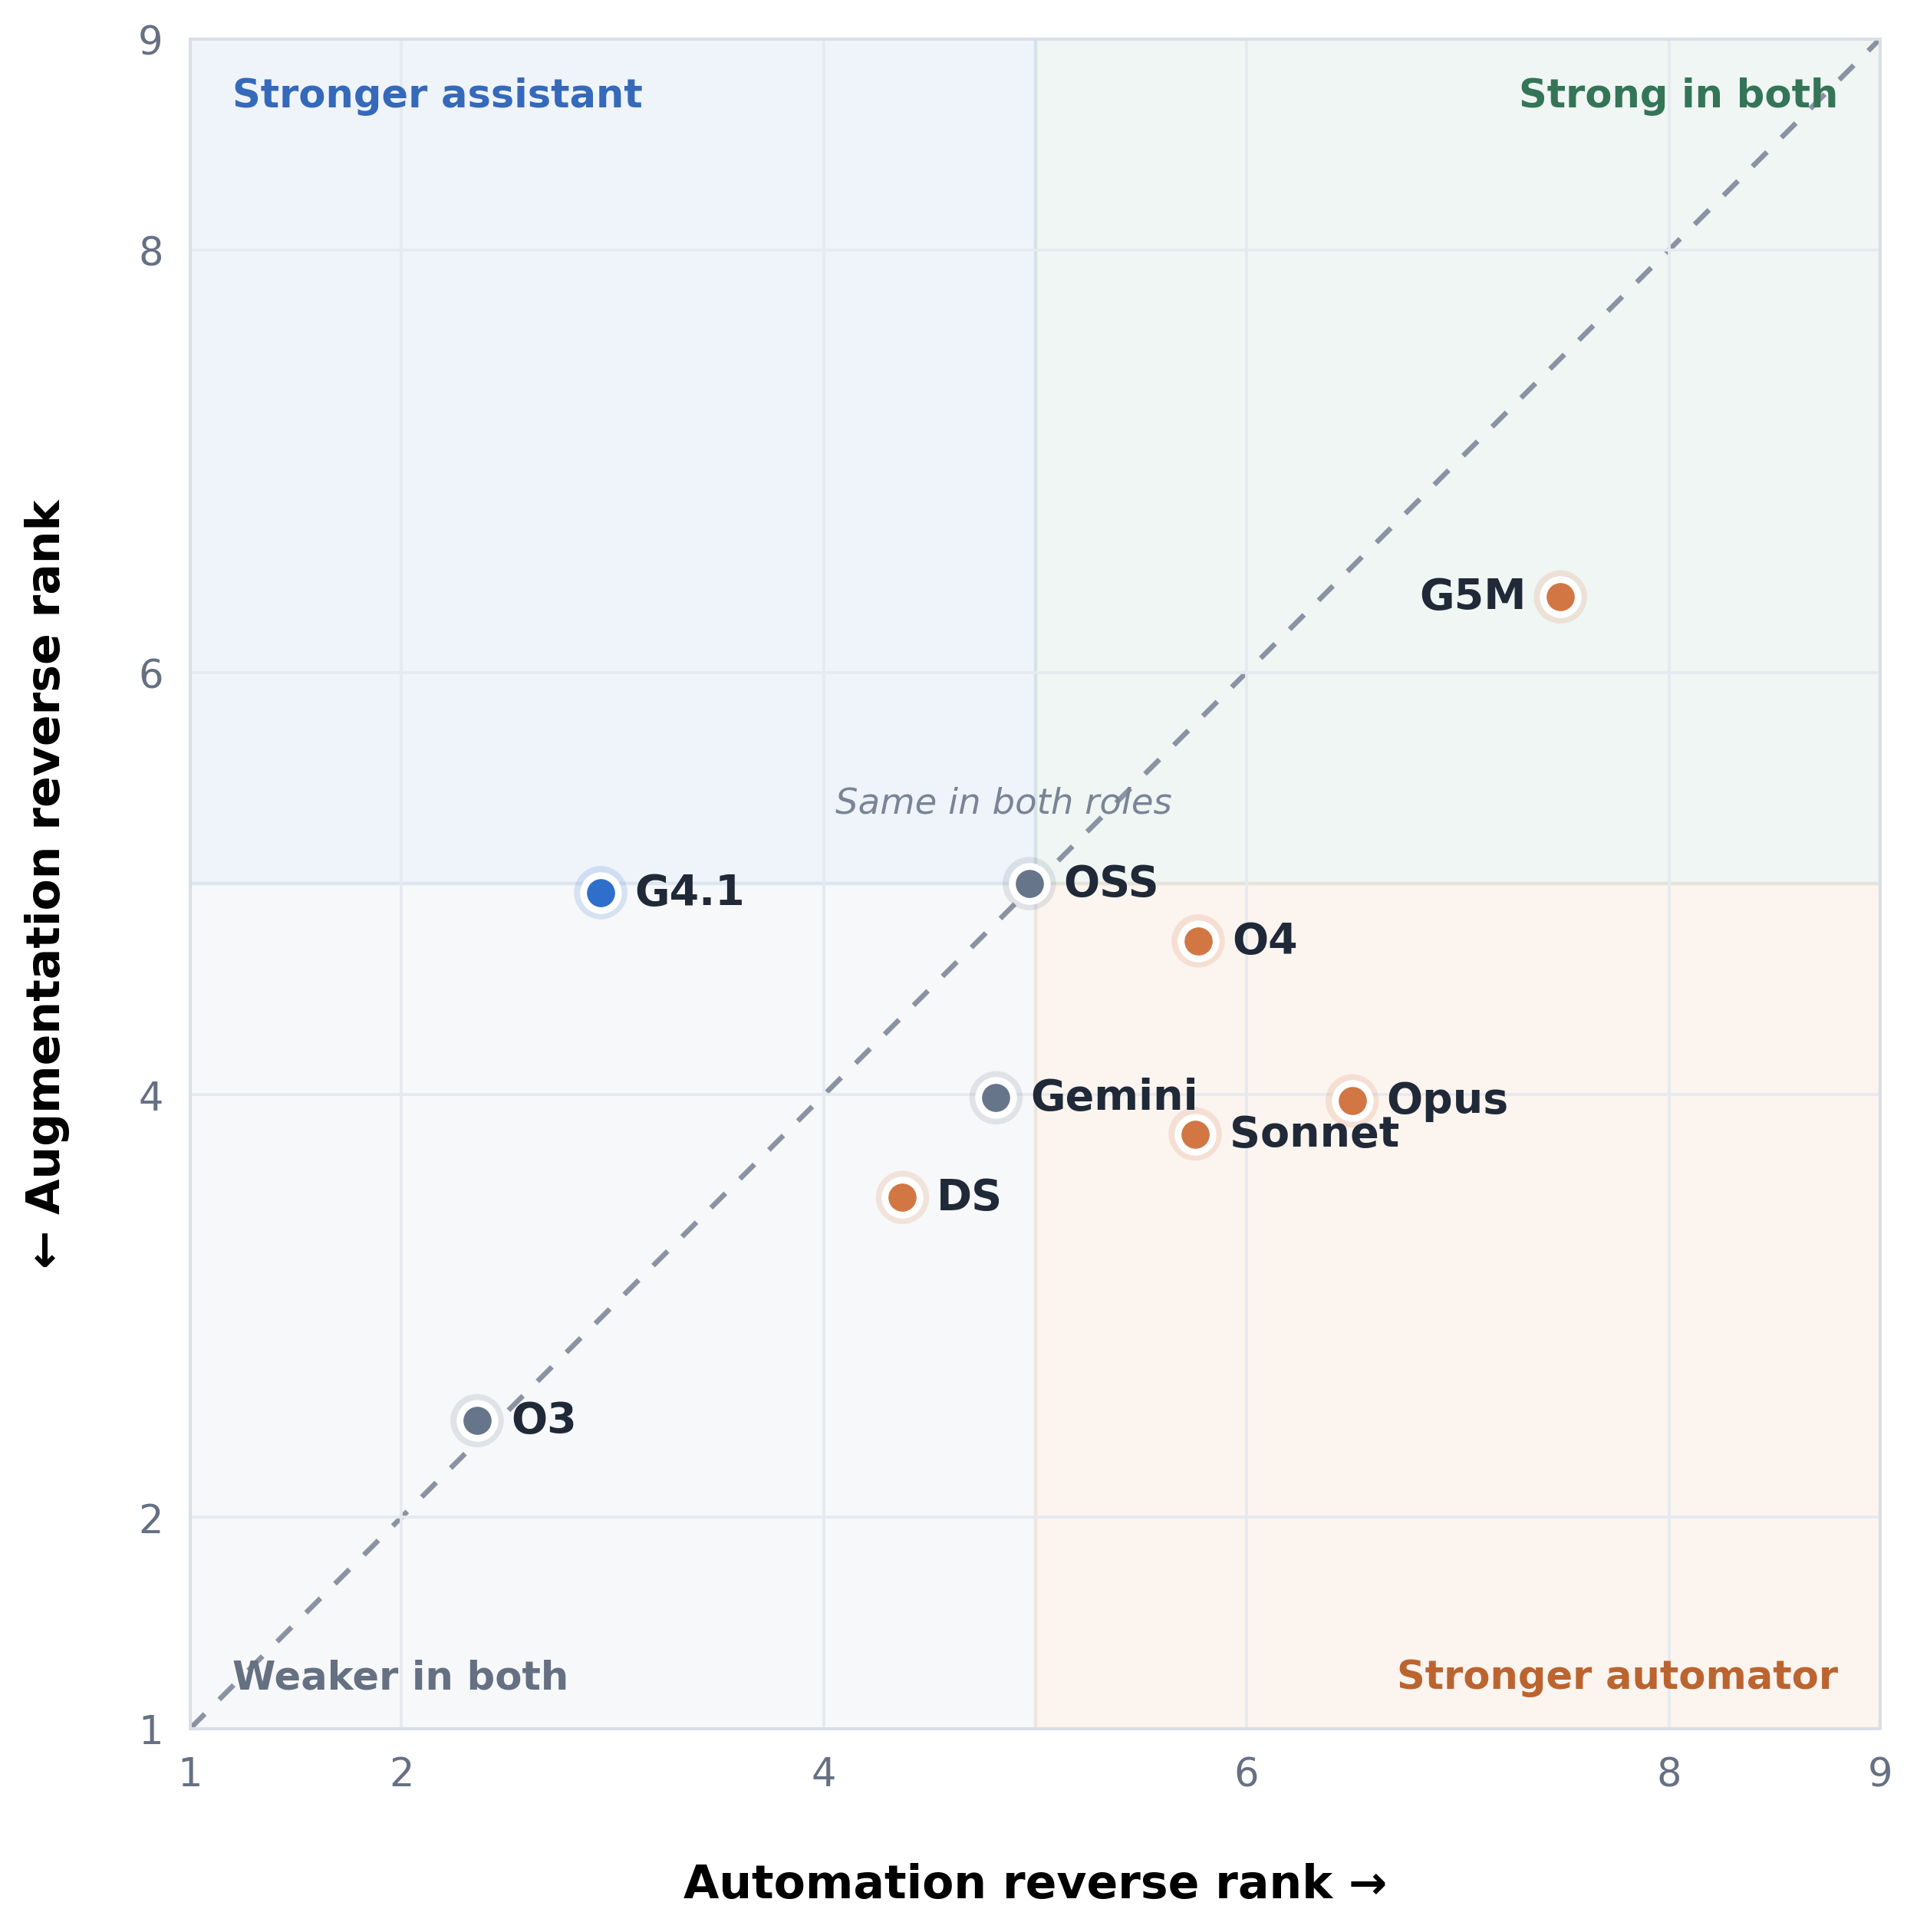
\includegraphics[width=0.79\linewidth]{figures/figure2b_role_swap_scatter_white.png}
    \caption{
    \textbf{Model-level comparison of average automation rank and average augmentation rank (assistant models only)}. 
    %Blue points report augmentation ranks and orange points report automation ranks; horizontal lines show the shift between regimes. Error bars show $\pm 1$ standard error, computed across ten independent runs after averaging ranks across tasks within each run. Lower rank indicates better performance.
    Each point represents one assistant model's average rank across seven tasks and ten independent runs. Ranks are inverted so that higher values indicate better performance. With nine assistant models, reverse rank is defined as \(10-\bar{r}\), where \(\bar{r}\) is the model's mean rank in the corresponding usage mode. The horizontal axis reports automation performance and the vertical axis reports augmentation performance. The unaided worker baseline is excluded.}
    \label{fig:role-swap-scatter}
\end{figure}

% Figure~\ref{fig:role-swap-scatter} compares each model's average automation rank and average augmentation rank. Several models move substantially across regimes. GPT-5-Mini is strong in both regimes and has the best average rank among assistant models in augmentation as well as the best average rank in automation. GPT-4.1 is relatively stronger as an assistant than as a direct solver: it ranks near the middle of the augmentation distribution but near the bottom in automation. Conversely, Claude-Opus-4.8, Claude-Sonnet-4.6, Gemini-3.1-Pro, and GPT-O4-Mini are stronger in automation than in augmentation. GPT-OSS-120B sits close to the diagonal, with similar average ranks across modes. The same model is thus not consistently favored when it solves a task directly versus when it assists another worker.

Figure~\ref{fig:role-swap-scatter} compares each model's average automation and augmentation rank. Across the nine shared assistant models, the Spearman rank correlation between automation and augmentation performance is moderate ($\rho=0.48$; two-sided $p=0.187$), but is not statistically distinguishable
from zero at conventional significance levels. GPT-5-Mini is strong in both usage modes and has the best average rank among assistant models in augmentation as well as the best average rank in automation. GPT-4.1 is relatively stronger as an assistant than as a direct solver. Conversely, Claude-Opus-4.8, Claude-Sonnet-4.6, Gemini-3.1-Pro, and GPT-O4-Mini are stronger in automation than in augmentation. GPT-OSS-120B sits close to the diagonal. Thus, automation performance contains some information about augmentation performance, but it is an incomplete proxy for it.


\begin{table}[htbp]
    \centering
    \small
    \begin{tabular}{lrr}
        \toprule
        Task & Spearman $\rho_t$ & $p$-value \\
        \midrule
        Tax Preparation & 0.85 & 0.004 \\
        Menu Planning & 0.64 & 0.066 \\
        Tutoring Session Planning & 0.50 & 0.166 \\
        Counseling & 0.25 & 0.516 \\
        Operations Research Analysis & 0.17 & 0.668 \\
        Market Trend Analysis & 0.10 & 0.798 \\
        Travel Planning & -0.04 & 0.915 \\
        \bottomrule
    \end{tabular}
    \caption{\textbf{Task-level correlation between automation and augmentation rankings.} Spearman correlations are computed across the nine assistant models using each model's mean rank over ten runs. Positive values indicate similar cross-mode ordering; values near zero indicate little correspondence. $p$-values are descriptive because each task contains only nine models.}
    \label{tab:mode-correlations}
\end{table}


The strength of this correlation varies substantially by task as shown by Table~\ref{tab:mode-correlations}. Tax preparation has the strongest cross-mode correlation ($\rho_{\mathrm{tax}}=0.85$), followed by menu planning ($\rho_{\mathrm{menu}}=0.64$) and tutoring ($\rho_{\mathrm{tutor}}=0.50$). The rankings are only weakly associated in counseling ($\rho=0.25$), operations research ($\rho=0.17$), and market trends analysis ($\rho=0.10$), and are essentially unrelated in travel planning ($\rho=-0.04$). Tax preparation is the only task whose association is statistically distinguishable from zero at the conventional level ($p=0.004$), including under a Bonferroni correction for seven task-level comparisons. Broader statistical significance across tasks would require a larger model pool or additional runs, and remains an avenue for future work.

The supplementary document's Table~\ref{tab:best-model-by-task} makes the divergence concrete. It reports the best-performing model in each task under automation and augmentation, using the lowest mean rank across ten runs. In five of seven tasks, the augmentation winner differs from the automation winner. In counseling, GPT-OSS-120B is the strongest automator while GPT-4.1 is the strongest assistant; in market-trends analysis, Claude-Opus-4.8 automates best but GPT-O4-Mini assists best; and in operations research, Gemini-3.1-Pro automates best while the unaided worker baseline ranks first in augmentation. Menu planning and tutoring are the two exceptions, where GPT-5-Mini ranks first in both usage modes.

The table also shows that augmentation winners are not uniformly frontier assistant models. GPT-3.5-Turbo (plain), the unaided worker with no external assistance, ranks first in operations research, tax preparation, and travel planning. Averaged across all seven tasks, the plain baseline has a mean rank
of $3.79$; GPT-5-Mini is the only assisted condition with a better overall mean rank of $3.66$. We read this not as evidence that guidance is futile, but as
evidence that its value is task-contingent and can be negative. Poorly matched or overly complex guidance can leave the worker worse off than working alone. The corollary is central to our argument that strong direct solvers do not automatically make strong assistants, and the right model depends jointly on the role it plays and the task it supports.

Lastly, several models exhibit large and reproducible
task-level role reversals. In market trends analysis, Claude-Opus-4.8 is the strongest automator (mean rank $2.05$) but one of the weakest assistants (mean rank $8.15$). Conversely, in counseling, GPT-4.1 ranks substantially better as an assistant (mean rank $3.80$, the best among assisted conditions) than as an automator (mean rank $7.40$). These differences persist after averaging across ten independent runs and therefore are not attributable to a single random run.

% seg into 4.4
The rankings establish that assistance quality is distinct from direct-solving ability, but they do not by themselves explain why particular assistance texts
help or hinder the downstream worker model. We therefore turn to the underlying assistance texts, worker outputs, rubric scores, and judge rationales. 
Section~\ref{sec:analysis} examines cases with especially large gaps between ranks to identify recurring differences between effective and ineffective assistance.

% The table also shows that augmentation winners are not uniformly frontier assistant models. GPT-3.5-Turbo (plain), the unaided worker with no external assistance, ranks first in operations research, tax preparation, and travel planning. We read this not as evidence that guidance is futile, but as evidence that its value is task-contingent and can be negative: poorly matched or overly complex guidance can leave the worker worse off than working alone. The corollary is central to our argument that strong direct solvers do not automatically make strong assistants, and the right model depends jointly on the role it plays and the task it supports. We interpret these qualitative differences in the guidance and final outputs in Section~\ref{sec:analysis}.

%% TODO - add a paragraph on correlations overall, and across tasks. (Done look above)

%% TODO - go back to the three results hihglighted in the intro and see that we covered all three (Checked)

%% TODO - we need an example for what is goiong on, either hre or start of next section

\subsection{Mechanisms: Preliminary Observations on Assistance Quality}
\label{sec:analysis}

To understand what traits make for effective augmentation, we turn to the education literature to ground our observational findings. \citet{wood1976}  coined the term ``scaffold'' to define the process that enables a learner to solve a task or achieve a goal that would be beyond their unassisted efforts. In their framing, as in ours, the expert guides the learner through a task rather than completing it for them. \citet{vandepol2010} take this concept further by identifying three essential properties of effective scaffolding: (1) contingency - support is calibrated to the learner's current level, (2) fading - support is gradually withdrawn as competence grows, and (3) transfer of responsibility - the goal is learner autonomy, not dependence. The first and third properties are most directly applicable to our single-interaction setting, where scaffolds cannot adapt over time. We apply this lens to our case in order to evaluate the LLM-generated assistance texts, which are analogous to the scaffolds in education. We compare the assistance texts received by the two highest-ranked outputs against those received by the two lowest-ranked outputs across all seven tasks. In doing so, we identify three characteristics of high-quality augmentation scaffolds.

%\begin{figure}[H]
\centering

\begin{minipage}[t]{0.485\textwidth}
\begin{tcolorbox}[
    enhanced,
    equal height group=or-assistance,
    colback=green!3,
    colframe=green!45!black,
    colbacktitle=green!45!black,
    coltitle=white,
    fonttitle=\bfseries\small,
    title={Higher-Ranked Assistance Text},
    boxrule=0.5pt,
    arc=2pt,
    left=6pt,
    right=6pt,
    top=5pt,
    bottom=5pt
]
\raggedright
\small
\textit{GPT-4.1, Operations Research, Run 2}

\medskip
\textbf{2.\ Plan and Structure}
\begin{itemize}
    \setlength{\itemsep}{3pt}
    \setlength{\parskip}{0pt}
    \item Outline a clear structure using logical headings aligned with each
    requirement.
    \item Allocate approximate word counts to each section to remain within
    the limit.
    \item Identify where to \textbf{highlight trade-offs and risk
    considerations in the recommendations}.
\end{itemize}

\textbf{3.\ Draft, Self-Review, and Finalize}
\begin{itemize}
    \setlength{\itemsep}{3pt}
    \setlength{\parskip}{0pt}
    \item \textbf{Ensure that all requirements are addressed and that the
    recommendations are balanced and well supported.}
\end{itemize}
\end{tcolorbox}
\end{minipage}
\hfill
\begin{minipage}[t]{0.485\textwidth}
\begin{tcolorbox}[
    enhanced,
    equal height group=or-assistance,
    colback=red!3,
    colframe=red!45!black,
    colbacktitle=red!45!black,
    coltitle=white,
    fonttitle=\bfseries\small,
    title={Lower-Ranked Assistance Text},
    boxrule=0.5pt,
    arc=2pt,
    left=6pt,
    right=6pt,
    top=5pt,
    bottom=5pt
]
\raggedright
\small
\textit{GPT-O3-Mini, Operations Research, Run 2}

\medskip
\textbf{2.\ Plan and Structure}
\begin{itemize}
    \setlength{\itemsep}{3pt}
    \setlength{\parskip}{0pt}
    \item Develop a high-level outline that organizes the content logically.
    \item Decide which headings could improve clarity.
    \item Integrate trade-offs and risks \textbf{without delving into specific
    solutions or analysis}.
\end{itemize}

\textbf{3.\ Draft, Self-Review, and Finalize}
\begin{itemize}
    \setlength{\itemsep}{3pt}
    \setlength{\parskip}{0pt}
    \item Finalize the document \textbf{without task-specific analytical
    content}.
\end{itemize}
\end{tcolorbox}
\end{minipage}

\caption{\textbf{Selected assistance-text excerpts for the operations research
task.} Intervening instructions are omitted for brevity. The higher-ranked
assistance text (left) directs the worker to address task requirements,
trade-offs, risks, and recommendations. The lower-ranked assistance text
(right) instead instructs the worker to avoid task-specific analysis, limiting
the usefulness of the resulting guidance.}
\label{fig:assistance-text-comparison}
\end{figure}

\begin{table}[htbp]
\centering
\definecolor{traitA}{RGB}{224,238,250} % soft blue
\definecolor{traitB}{RGB}{255,247,222} % soft yellow
\definecolor{traitC}{RGB}{250,228,228} % soft rose
\footnotesize
\setlength{\tabcolsep}{5pt}
\renewcommand{\arraystretch}{1.25}
\begin{tabularx}{\linewidth}{
    >{\raggedright\arraybackslash}p{1.0cm}
    >{\raggedright\arraybackslash}p{3.0cm}
    >{\raggedright\arraybackslash}X}
\toprule
 & \textbf{Task, assistant (rank)} & \textbf{Assistance-text excerpt} \\
\midrule

% run 4
\rowcolor{traitA} \multicolumn{3}{l}{\textbf{Trait 1: Specificity beyond the prompt (contingency)}} \\
\rowcolor{traitA} \textbf{Good} & Market trends, GPT-5-Mini (1) &
``For each trend, plan 2 to 3 succinct bullets: core observation, primary driver(s), and potential market implication\ldots a short preface about methodology and data vintage.'' \\
\rowcolor{traitA} \textbf{Bad} & Market trends, GPT-4.1 (9) &
``Ensure you understand the expectation to discuss how various factors (supply, demand, weather, storage, LNG exports, infrastructure, policy) interact\ldots'' \textit{(restates the prompt's factor list)} \\
\addlinespace

% run 1
\rowcolor{traitB} \multicolumn{3}{l}{\textbf{Trait 2: Explicit structure and ordering}} \\
\rowcolor{traitB} \textbf{Good} & Travel planning, Gemini-3.1-Pro (3) &
Enforces assumptions and clarifying questions ``\emph{before} the provisional itinerary,'' with named sections in explicit order: Introduction $\to$ Budget Breakdown $\to$ Daily Itinerary $\to$ Conclusion. \\
\rowcolor{traitB} \textbf{Bad} & Travel planning, GPT-O4-Mini (9) &
``Determine sequence and hierarchy of information for clarity and flow''; instructs worker to ``populate each section with neutral placeholders\ldots\ \emph{[Day 1: transportation placeholder]}''; no ordering is prescribed. \\
\addlinespace

% run 2
\rowcolor{traitC} \multicolumn{3}{l}{\textbf{Trait 3: Not working against the task}} \\
\rowcolor{traitC} \textbf{Good} & Operations research, Gemini-3.1-Pro (3) &
``Present two distinct, practical strategies. For each, explicitly state the expected benefits, potential drawbacks, and associated risks.'' \\
\rowcolor{traitC} \textbf{Bad} & Operations research, GPT-O3-Mini (9) &
``Establish a workflow for integrating\ldots trade-offs \textbf{without delving into specific solutions or analysis}''; finalize ``\textbf{without\ldots task-specific analytical content}.'' \\
\addlinespace

\bottomrule
\end{tabularx}
\caption{\textbf{Illustrative higher- vs.\ lower-ranked assistance texts for each
scaffold-quality characteristic.} Rows are color-coded by trait; ranks are the aggregate
augmentation rank within the task run. Excerpts are drawn from the assistance texts and lightly trimmed.}
\label{tab:trait-examples}
\end{table}


First, good guidance includes specificity that adds analytical value beyond the prompt, rather than just regurgitating information from the prompt, which is an application of the contingency principle, where effective scaffolding is calibrated to the learner's specific challenge rather than offered generically \citep{vandepol2010}. Table~\ref{tab:trait-examples} illustrates each trait with a higher- and lower-ranked assistance text. Low-performing guidance messages that simply echo the prompt's own constraints do not augment the focal worker, who already have access to the prompt. For example, in the market trends task, a top assistance text directs the worker to pair each trend with its primary driver and likely market implication and to note the underlying methodology, whereas a bottom-tier assistance text merely restates the prompt's own list of factors without adding an analytical step.

Next, embedding explicit structural requirements into the workflow is another trait of a top assistance text. In the travel planning task, a top assistance text enforces assumptions and clarifying questions before the provisional itinerary and prescribes a named section sequence (introduction, budget breakdown, day-by-day itinerary, and conclusion), making the ordering non-negotiable. A bottom-tier assistance text, by contrast, delegates ordering to the worker by instructing it to ``determine sequence and hierarchy of information for clarity and flow,'' and substitutes neutral placeholders for actual structural guidance.

Third, a negative point that good scaffolds avoid: actively working against task completion. Effective scaffolding includes what \citet{wood1976} term \textit{direction maintenance}, keeping the learner oriented toward the task objective. The most harmful assistance texts in our study invert this function entirely: rather than correcting learner drift, the scaffold itself redirects the worker away from the core deliverable, by instructing the worker not to finish the task as described in the prompt. In operations research task, a bottom ranked scaffold instructs the worker to establish a workflow for integrating necessary performance indicators, risk discussions, and balanced trade-offs without delving into specific solutions or analysis, yet the task explicitly requires two practical solutions with trade-offs stated. This instruction directly prohibits the core deliverable. Thus, no assistance can often beat bad assistance. Notably, the unaided worker is a strong baseline: the plain condition (GPT-3.5-Turbo with no assistance) ranks at or near the top in the many tasks. Poorly calibrated assistance is therefore frequently worse than none, undermining the transfer of responsibility that effective scaffolding aims to achieve \citep{vandepol2010}.

% OLD
%For tasks that require domain knowledge, such as tax law, a heavy assistant text that introduces caveating language or irrelevant processes can push the worker below its unassisted baseline. In fact, the plain condition (no assistance) tops the rankings for tax preparation. Extraneous advice, such as noting that gaps may prevent exact liability calculations, can be distracting or suggest hedging behavior, rather than letting the worker apply its own tax knowledge. This type of augmentation undermines the transfer of responsibility that effective scaffolding aims to achieve \citep{vandepol2010}.


\section{Discussion}

    
Our results show that automation and augmentation are not two labels for the same underlying capability. They produce systematically different rankings. The top-ranked model differs between automation and assistant-only augmentation in five of the seven tasks. Thus, the assistant value is sharply task-contingent. Interpreting these patterns requires moving beyond leaderboard thinking to role-specific model selection. The automation results are comparatively concentrated around a small set of
direct solvers, while GPT-3.5-Turbo ranks last. This ordering characterizes performance on our single-turn professional deliverables and should not be interpreted as reproducing the orderings of agentic benchmarks built
around multi-step tool use and environment interaction.
Augmentation tells a different story. No single model dominates across tasks, average ranks are more dispersed, and several strong direct solvers perform poorly as assistants. Most strikingly, on operations research, tax preparation, and travel planning, the unaided GPT-3.5-Turbo worker outranks every assisted condition, and it has the second best average augmentation rank overall after GPT-5-Mini. We read this not as evidence that assistance is useless, but as evidence that its value is conditional and can be negative. Poorly matched or overly complex process guidance can distract the worker, constrain useful execution, or push it away from task requirements.

\subsection{Implications for Organizations and Workflow Design}

Our framework offers several practical applications for individuals and organizations adopting AI systems. First, it can support model selection across teams, products, and workflows. Teams seeking a reliable solver for well-defined, repeatable tasks may prioritize automation performance, whereas teams embedding AI into expert workflows, where the goal is to improve human output rather than replace human judgment, may prioritize augmentation ability.

Importantly, the framework is modular. In our experiments, we use GPT-3.5-Turbo as an illustrative fixed worker model to demonstrate the pipeline and hold the worker role constant across augmentation trials. However, individuals and organizations can substitute this worker model with a model, human baseline, or internal workflow proxy that better reflects their own deployment context. For example, a consulting firm could evaluate how different assistant models guide junior analysts, domain experts, customer-support agents, or a preferred internal model. This flexibility allows the framework to be adapted to local goals, constraints, and performance standards.
    
Secondly, designing human-AI collaboration can be done more efficiently and effectively. Beyond model selection, our framework can guide how organizations structure the division of labor between humans and AI. At the organizational level, different models can be assigned to different subtasks according to where each model's comparative advantage lies. At the team level, human-AI pairs can use the automation/augmentation profiles to decide which subtasks to delegate entirely versus which to treat as collaborative, keeping humans in the loop where an assistance yields the largest gains. At the individual level, a practitioner can use the same logic to choose the tool best matched to their specific workflow, rather than defaulting to a single general-purpose assistant.

\subsection{Implications for Evaluation and Research}

Our findings also speak to how LLMs should be evaluated. Many existing benchmarks measure automation almost exclusively. If gains on those benchmarks do not transfer to augmentation, then labs and leaderboard builders may be optimizing for only one economically relevant capability. Adopting automation and augmentation as distinct evaluation axes would make model profiles more informative for human-in-the-loop and multi-agent deployment. If automation and augmentation are empirically distinct capabilities, then any evaluation that tests only one is incomplete by design, and our framework offers a template for fixing that. Leaderboard builders and AI labs optimizing for benchmark performance could adopt the automation vs. augmentation distinction as a structural requirement for capability evaluation.
    
CentaurBench sits between two literatures. Relative to large CS benchmarks, it evaluates economically grounded occupational tasks under a fixed coaching protocol rather than abstract capability alone. Relative to field experiments, it compares many frontier models across both roles and multiple domains rather than a single tool in a single setting. Relative to marketplace benchmarks such as HAPI \citep{upwork_hapi2025}, it holds the downstream worker fixed to isolate assistant quality across models at scale. The appropriate next step is not to replace one paradigm with another, but to combine them for optimal model selection. 

% rephrased above
%The last application is a meta one. We believe that our framework is itself a critique of how models are currently benchmarked. Researchers building leaderboards, and AI labs deciding what to optimize for, could use the automation/augmentation distinction as a structural requirement for any serious capability evaluation. The implicit argument is that existing benchmarks are incomplete by design, and our framework offers a template for fixing that.

    
\subsection{Limitations and Future Work}

    % This study should be read as an initial introduction of the simulation framework and a pilot evaluation, not as a definitive mapping of model capabilities across tasks and usage regimes. The results identify where distinctions between automation and augmentation appear most and provide preliminary model profiles that can guide subsequent empirical validation. Because the current evaluation relies on LLM judges, the findings should be interpreted as scalable simulation evidence rather than definitive human expert judgments. Validating a subset of tasks with domain experts remains a priority, particularly to assess whether assistant advantages observed in simulated settings persist in authentic workplace contexts.

This study introduces a simulation and evaluation framework to measure models' ability to augment and automate tasks across usage modes. We present this as an initial pilot application; it should not be interpreted as a definitive mapping
of model capabilities across tasks and usage modes. The results identify
settings in which automation and augmentation rankings diverge and provide
preliminary model profiles for subsequent validation. More broadly, the study
motivates the development of assistance-oriented benchmarks rather than
claiming to provide a comprehensive benchmark itself.

Because the current evaluation relies on LLM judges, the findings constitute
scalable simulation evidence rather than definitive human or domain-expert
judgments. Although we use general and task-specific rubrics, multiple judges,
leave-family-out evaluation, and repeated runs, these procedures cannot eliminate all evaluator bias. Human validation remains a priority, particularly for tasks such as counseling, tax preparation,
tutoring, and operations research, where domain expertise and professional
judgment are consequential to assess whether assistant advantages observed in simulated settings persist in authentic workplace contexts.

Several extensions are especially important. First, the present design evaluates augmentation through a single assistance text passed to a fixed worker. Real professional workflows are often iterative: assistants clarify requirements,
revise plans, and respond to feedback across multiple turns. Extending the
framework to multi-turn and agentic settings, in which an assistant contributes
throughout an evolving workflow rather than through one-shot guidance, is a
natural next step.

Second, all augmentation conditions use the same worker model, GPT-3.5-Turbo. Holding the worker fixed isolates variation in the assistance
provided, but it also limits generalizability. Guidance that helps one worker may not transfer to another. A stronger or differently aligned worker may need less assistance, while a weaker worker may benefit more from structured
guidance. Future studies should vary worker capability and model family to test
whether assistant rankings remain stable across downstream worker models.

Third, the pilot includes seven professional tasks and ten independent
generation-and-evaluation runs. Replication improves the stability of the
reported estimates, but the task set remains modest relative to the diversity
of real-world, occupational tasks. Expanding the evaluation to additional tasks, industries, risk levels, and deliverable formats would provide stronger evidence about the generalizability of role-specific model performance.


External validation should combine domain expertise with authentic workplace
tasks. Upwork's Human+Agent Productivity Index (HAPI) \citep{upwork_hapi2025}, for example, emphasizes verified marketplace
deliverables and human rubric scoring. Our design instead holds the downstream
worker fixed to isolate differences in assistance quality across models at
scale. Future work could combine these strengths by using workplace-grounded
tasks, validating a preregistered subset with domain experts, and explicitly
comparing automation and augmentation rankings. This would establish whether
the preferences of LLM judges correspond to expert assessments of final-output quality, guidance usefulness, and workplace value.

% Equally important is external validation with human experts and, where appropriate, human-subject studies or deployment-oriented case studies. In Upwork's Human+Agent Productivity Index (HAPI) \citep{upwork_hapi2025}, collaboration with human experts on verified marketplace deliverables and human rubric scoring is a highlighted component of the experiment. Our framework instead holds the downstream worker fixed to isolate assistant quality across frontier models at scale. A priority for future work is combining these strengths, from marketplace-grounded tasks, human validation on a subset, and explicit automation-augmentation ranking for model selection. Such validation would help determine whether pairwise LLM-judge rankings align with expert assessments of output quality, guidance usefulness, and real-world utility.

%The best mathematicians are not necessarily the best mathematics teachers, and the highest-ranked tennis players are not necessarily the best coaches. As AI systems increasingly advise humans and coordinate with other models, we need to develop a more robust way to evaluate not only a model's ability to automate tasks, but also its capability to augment them. This study offers an initial framework for making that distinction measurable and motivates a broader evaluation agenda organized around the role a model plays, the worker it supports, and the task they jointly perform. More generally, many have called for a world where AI systems do not automate human work, but instead support human flourishing by augmenting our capabilities to superhuman levels. If this dream is to be achieved, efforts like CentaurBench offer one small step in reframing the conversation on what the future of AI progress should look like. 

The best mathematicians are not necessarily the best mathematics teachers, and the highest-ranked tennis players are not necessarily the best coaches. As AI
systems increasingly advise humans and coordinate with other models, evaluation
must measure not only a model's ability to automate tasks, but also its capacity
to augment the performance of others. This study offers an initial framework
for making that distinction measurable and motivates a broader evaluation
agenda organized around the role a model plays, the worker it supports, and the
task they jointly perform. 

More broadly, realizing the potential of AI to complement human judgment, expand human capability, and support human
flourishing will require measures of progress that extend beyond autonomous
task completion. Our framework represents one step towards reframing AI
progress around not only what systems can accomplish independently, but also
how effectively they enable humans and other agents to accomplish even more.


%%%%%%%%%%%%%%%%%%%%%%%%%%%%%%%%%%%%%%%%%%%%%%%%%%%%%%%%%
%\newpage

\bibliographystyle{aaai2027}
\bibliography{references}

%%%%%%%%%%%%%%%%%%%%%%%%%%%%%%%%%%%%%%%%%%%%%%%%%%%%%%%%%
\end{document}
